\documentclass[12pt]{article}

% ============================================================
% PACKAGES
% ============================================================

\usepackage{amsmath}
\usepackage{amssymb}
\usepackage{amsthm}
\usepackage{mathtools}
\usepackage{bm}
\usepackage{bbm}

\usepackage{booktabs}
\usepackage{threeparttable}
\usepackage{multirow}
\usepackage{array}
\usepackage{graphicx}
\usepackage{adjustbox}
\usepackage{placeins}
\usepackage{float}
\usepackage{subcaption}

\usepackage[margin=1in]{geometry}
\usepackage{setspace}
\onehalfspacing

\usepackage[authoryear,round]{natbib}

\usepackage[
    colorlinks=true,
    citecolor=blue,
    linkcolor=blue,
    urlcolor=blue
]{hyperref}

\usepackage{enumitem}
\usepackage{xcolor}
\usepackage{microtype}

% ============================================================
% THEOREM ENVIRONMENTS
% ============================================================

\newtheorem{proposition}{Proposition}
\newtheorem{lemma}{Lemma}
\newtheorem{corollary}{Corollary}
\newtheorem{assumption}{Assumption}

\theoremstyle{definition}
\newtheorem{definition}{Definition}

\theoremstyle{remark}
\newtheorem{remark}{Remark}

% ============================================================
% CUSTOM COMMANDS
% ============================================================

\newcommand{\E}{\mathbb{E}}
\newcommand{\Var}{\operatorname{Var}}
\newcommand{\Cov}{\operatorname{Cov}}
\newcommand{\Prob}{\mathbb{P}}

\newcommand{\argmax}{\operatorname*{arg\,max}}
\newcommand{\argmin}{\operatorname*{arg\,min}}

% ============================================================
% TITLE
% ============================================================

\title{Optimal Pricing with Preferences for Product Switching}
\author{Tate Mason}
\date{\today}

 %============================================================
% DOCUMENT
 %============================================================

\begin{document}

\maketitle

\begin{abstract}
  INSERT ABSTRACT
\end{abstract}

\newpage

% ============================================================
% INTRODUCTION
% ============================================================

\section{Introduction}
\label{sec:introduction}

Consumers face repeated choice problems frequently in daily life. The decision of what to buy at the grocery store, what TV show to watch, or what to order at a restaurant all constitute a choice problem which relies on past decisions to inform current consumption decisions. A consumer who habitually consumes the same dish at their favorite restaurant may exhibit dynamic preferences for this dish. Similarly, one could imagine the opposite case, where a consumer orders a new dish having grown fatigued of their usual order. These examples describe cases in which dynamic consumption patterns and dynamic preferences influence consumption.

Dynamic preferences are not just important to the consumer - the firm can also utilize them to maximize profits. Product introduction problems, price discrimination, or bundling decisions can all be influenced by the internalization of dynamic preferences. Price discrimination especially is easy to imagine: a firm sets lower prices to induce a habitual consumer to purchase their good, then take advantage of their state dependence by raising prices. This price discrimination context is the lens through which I analyze how the firm and consumers are impacted by dynamic switching preferences.

I examine the value of information on consumer types by solving a two-period theoretical model for optimal pricing and profit. Using Nielsen HomeScan and MarketScan data, I estimate flavor-switching preferences and heterogeneous price sensitivity, then use those estimates to price plain yogurt against all other choices. I use the estimates to quantify how knowledge of switching type affects revenue and consumer welfare.

I find consumers exhibit little preference for switching, though there is a wide distribution of types. I find that the consumer is not unilaterally disadvantaged by price discrimination. For the initially inside consumer, total welfare increases for all but the tails of the switching-type distribution. For the initiall outside consumer, only the highest switching-type consumer sees total welfare decreases. Almost all total welfare effects are driven by consumer welfare effects. 


% ============================================================
% BACKGROUND AND LITERATURE
% ============================================================

\section{Related Literature and Contribution}
\label{sec:literature}

SUPPLY LITERATURE - TARGETED PRICING AND STATE DEPENDENCE
DEMAND LITERATURE - ESTIMATION OF PREFERENCES AND MODELING

CONTRIBUTION - TYPE DISTRIBUTION, FIRM PRICING OFF TYPE



% ============================================================
% THEORETICAL SUPPLY SIDE
% ============================================================

\section{Theoretical Framework}
\label{sec:theory}

There is a singular monopolist firm in the market who produes a single good $j$. There are a continuum of consumers $\mathcal{N}$ who will live for two periods, deciding on a purchase decision $h_t \in \{j, 0\}$, choosing between the monopolist good or the outside option, any other good. Consumers enter the model with a type $r = \{H, L\}$ which informs whether they have high or low preference for switching $\gamma_r$. They also enter with an initial purchase state $h_0 = \{j, 0\}$, describing their last purchase before being seen by the firm.

In the baseline specification, the firm is aware of each consumer's switching type $\gamma_r$ and initial history $h_0$. They will use this information to price discrminate according to different combinations of type and history.

\subsection{Consumer Demand}
\label{subsec:model-demand}

Let consumer utility be defined as follows:
\begin{equation}
  u_t(h_t\mid h_{t-1},\gamma_r) = \mathbbm{1}\{h_t=j\}(\beta+\alpha p_t(h_{t-1}, \gamma_r)) + \gamma_r\mathbbm{1}\{h_t\ne h_{t-1}\} + \varepsilon_{h_t, t}, \ \alpha < 0
\end{equation}
  
Here, $\beta$ is baseline utility from the inside option, $\alpha$ is homeogeneous price sensitivity, $p_t(h_{t-1}, \gamma)$ is the type and history specific price set by the firm, $\gamma_r$ captures switching utility, and $\varepsilon_{h_t, t}$ is the Type-I extreme value shock. Thus, if a consumer remains on a product $j$ for multiple periods, they do not enjoy the switching utility. This means the outside option gains utility of $\gamma_r$ if the consumer switches from inside option to outside option between periods. 

Given the Type-I extreme value shock, we can write choice probabilities in the form:

\begin{align}
  P_{h_t}(p_{h_{t-1}, \gamma_r}, \gamma_r) &= \frac{\exp\{v_{h_t}(p_{h_{t-1}, \gamma_r})\}}{1 + \exp\{v_{h_t}(p_{h_{t-1}, \gamma_r})\}}, \\
  q(h_t) &= 
  \begin{cases}
    -1, & h=j,\\
    1, & h=0.\\
  \end{cases}
   \\ v_h &= \beta + \alpha p_t(h_{t-1}, \gamma_r)+\gamma_rq(h_{t-1})
\end{align}

From the differencing of deterministic value for consumers, consumers experience a switching cost if they continue to consume the inside good and a switching boost if they switch in from the outside good. We can write the inside share as equivalent to the choice probability:

\begin{align*}
  s_{r, t}(h_{t-1}) = P_{H_t=j\mid h_{t-1}=h, \gamma_r, p_t(h_{t-1}, \gamma_r)} \\
\end{align*}

The outside share is equivalent to $1 - s_{r,t}(h_{t-1})$. Taking the derivative with respect to prices and switching utility will yield the price and switching elasticities:
\begin{align*}
  \frac{\partial s_{r, t}(h_{t-1})}{\partial p_t(h_{t-1}, \gamma)} &= \alpha s_{r,t}(h_{t-1})(1-s_{r,t}(h_{t-1})) \\
  \frac{\partial s_{r,t}(h_{t-1})}{\partial\gamma} &= q(h_{t-1})s_{r,t}(h_{t-1})(1-s_{r,t}(h_{t-1}))
\end{align*}


\subsection{Firm's Problem}
\label{subsec:firm-problem}
Let $h_0$ be the initial choice and $h_1$ the realized first-period choice.
All profits below are per consumer, conditional on the firm-observed type and initial state.
Marginal cost $c$ is fixed, and prices $p_{t}(h_{t-1}, \gamma)$ are nonnegative. The main-text benchmark sets $\delta=1$. For ease of notation, I will forego the $r$ subscripts. 

Define the firm's per-period profit function as follows:

\begin{align}
  \pi_1 &= s_1(h_0)[p_1(h_0, \gamma)-c], \\
 \pi_2(h_1)&=\max_{p_2(h_1, \gamma)\geq 0}s_2(h_1)[p_2(h_1,\gamma)-c],
 \qquad \Delta \pi_2=\pi_2(j)-\pi_2(0),\\
\end{align}

The firm maximizes second period profits $\pi_2$ by choosing an optimal price given period-one choice $h_1$ and consumer type $\gamma$. This terminal condition allows us to derive the total profit function for the firm:

\begin{align}
\Pi(p_1(h_0, \gamma);h_0)&=s_1(h_0)(p_1(h_0,\gamma)-c)
 +\{s_1(h_0)\pi_2(j)+[1-s_1(h_0)]\pi_2(0)\}\notag\\
 \label{eq:supply-profit}\\
\end{align}

The firm's total profit is composed of period-one profit and a continuation term which accounts for both potential states of the world in period-two given a consumer's initial state $h_0$. Thus, the firm must weigh their future prospects when setting period one prices, maximizing expected profit through period-two prices. 

\begin{align}
 \Pi^*(h)&=\max_{p_1(h)\geq 0}\Pi(p_1;h).
\end{align}

\section{Optimal Pricing}
\label{sec:optimal-pricing}

Derivation of optimal pricing conditions requires solving for period-two's optimal price first before deriving period-one's. Let $s_t$ be the inside share and $1-s_t$ be the outside share for $t=\{1,2\}$.

\label{subsec:foc}
For each realized first-period choice $h_1\in\{j,0\}$,
\begin{align}
0&=s_2+\alpha s_2(1-s_2)(p_2(h_1)-c),\\
 p_2^*(h_1)&=c-\frac{1}{\alpha[1-s_2^*(h_1)]}.
 \label{eq:supply-terminal}
\end{align}
The corresponding continuation value is
\begin{equation}
 \pi_2(h_1)=-\frac{s_2^*(h_1)}{\alpha[1-s_2^*(h_1)]}.
\end{equation}

\subsection{Period One}
\label{subsec:price-derivation}
With $\Delta \pi_2=\pi_2(j)-\pi_2(0)$,
\begin{align}
  0&=s_1+\alpha s_1(1-s_1)[p_1(h_0)-c+\Delta \pi_2],\\
  p_1^*(h_0)&=c-\frac{1}{\alpha(1-s^*_1(h_0))}-\Delta \pi_2.
 \label{eq:supply-first}
\end{align}
Expected profit at the optimum is
\begin{equation}
  \Pi^*(h)=\pi_2(0) - \frac{s^*_1(h_0)}{\alpha(1-s^*_1(h_0))}.
\end{equation}
These pricing equations and the comparative statics below apply at interior optima. When the price constraint binds, the optimal price is zero and profit is evaluated at that offer.
Full derivations are in Appendix~\ref{app:supply}.

\section{Comparative Statics}
\label{sec:comparative-statics}

To describe how prices and profits react to changes in $\gamma$ I derive the derivatives of different objects with respect to $\gamma$. Firstly, understanding how prices will respond to fluctuations in $\gamma$ is particularly important.

%\begin{proposition}
  Prices respond to $\gamma$ differently given previous purchase state $h_{t-1}$.
%\end{proposition} 

\begin{align}
  \frac{dp_2^*(h_1)}{d\gamma} &= -\frac{q(h_1)s_2^*(h_1)}{\alpha}, \\
  \frac{dp_1^*(h_0)}{d\gamma} &= -\frac{q(h_0)s_1^*(h_0) + (1-s_1^*(h_0))[s_2^*(j) + s_2^*(0)]}{\alpha}
 \label{eq:supply-gamma-prices}
\end{align}

The above conditions indicate distinct pricing responses given history and switching type. As switching preferences increase, period-two prices increase following an outside purchase and decrease following an inside purchase. In period one, stronger switching preferences raise the price for consumers who start outside. At a given price, these consumers are more willing to buy the inside good, giving the firm less incentive to lower the prices to encourage an inside purchase as doing so leaves the consumer more inclined to switch out in period two. For those who are initially inside, pricing moves in opposite directions. Stronger switching preferences lowers the willingness to pay for the inside good at a given price, while reduced incentive to encourage an inside purchase drives prices up. Thus, the net effect on period-one prices is ambiguous.

Profit's respons to $\gamma$ is also history dependent, given by

\begin{align}
  \frac{d\Pi^*(h_0)}{d\gamma} &= \frac{-q(h_0)s_1^*(h_0) + [s_1^*(h_0)s_2^*(j) - (1-s_1^*(h_0))s_2^*(0)]}{\alpha}
\end{align}

From the above, profit will display different responses to changes in $\gamma$ by initial state $h_0$. For someone who is initially outside, profits increase with $\gamma$ as the probability of a period one purchase rises at a given price. The resulting profit gain outweighs the decline in continuation profit following an inside purchase, so expected profit increases. For the inside consumer, we again see an ambiguous effect. Stronger switching preferences reduce the probability of a period-one purchase at a give price. Expected profit only rises if the gain in continuation profit following an outside purchase outweighs the losses from lower period-one demand and the decline in continuation profit following an inside purchase.

For each purchase path $(h_0,h_{t-1})\in\{(0,0),(0,j),(j,j),(j,0)\}$ such that $p_2^*(h_1)\ne0$,

\begin{align}
 R(h_0,h_1)&=\frac{p_1^*(h_0)}{p_2^*(h_1)},\\
 \frac{dR(h_0,h_1)}{d\gamma} &=\frac{p_2^*(h_1)\frac{dp_1^*(h_0)}{d\gamma}-p_1^*(h_0)\frac{dp_2^*(h_1)}{d\gamma}}{[p_2^*(h_1)]^2}
\end{align}

To illustrate $\gamma$'s effect on $R(h_0, h_1)$, we can look at how it varies with different consumption states. Take, for instance, $R(0,j)$; here, the price ratio increases with $\gamma$ because the first-period price increases and second-period decreases, as found in the pricing conditions. Thus, as $\gamma$ increases, the firm recognizes the need to extract value in period-one before lowering period-two prices to incentivize continued purchasing of the inside good. 

%\subsection{Numerical Supply Results}
%\begin{equation*}
% \beta=2,\qquad\alpha=-1,\qquad\delta=0.92,\qquad c=0,
% \qquad\gamma\in[-3,3].
%\end{equation*}
%\begin{table}[htbp]
%\centering\small
%\caption{Selected optimal prices and profits in the theoretical supply model}
%\label{tab:supply-solutions}
%\begin{tabular}{crrrrrr}\toprule
%  $x_0$ & $\gamma$ & $p_1^*$ & $p_2^*(j)$ & $p_2^*(0)$ & $\Pi^*$ & $\Pi^{*\prime}$\\\midrule
%  $j$ & -3 & 3.395 & 3.926 & 1.120 & 5.087 & -1.387\\
%  $j$ & -1 & 2.236 & 2.557 & 1.567 & 2.669 & -0.959\\
%  $j$ & 0 & 2.000 & 2.000 & 2.000 & 1.920 & -0.500\\
%  $j$ & 1 & 2.209 & 1.567 & 2.557 & 1.731 & 0.125\\
%  $j$ & 3 & 3.592 & 1.120 & 3.926 & 2.702 & 0.668\\
%  $0$ & -3 & -0.780 & 3.926 & 1.120 & 0.913 & 0.195\\
%  $0$ & -1 & 1.045 & 2.557 & 1.567 & 1.478 & 0.385\\
%  $0$ & 0 & 2.000 & 2.000 & 2.000 & 1.920 & 0.500\\
%  $0$ & 1 & 2.956 & 1.567 & 2.557 & 2.478 & 0.615\\
%  $0$ & 3 & 4.801 & 1.120 & 3.926 & 3.912 & 0.804\\
%  \bottomrule\end{tabular}
%\end{table}
%\FloatBarrier
%\begin{figure}[htbp]
%\centering
%%\includegraphics[width=\linewidth,height=.65\textheight,keepaspectratio]{assets/results/supply/optimal_prices_by_gamma.pdf}
%\caption{Optimal prices by switching preference and initial state}
%\label{fig:supply-prices}
%\end{figure}
%\FloatBarrier
%\begin{figure}[htbp]
%\centering
%%\includegraphics[width=\linewidth,height=.65\textheight,keepaspectratio]{assets/results/supply/all_state_realized_profit.pdf}
%\caption{Profit conditional on initial state and first-period choice}
%\label{fig:supply-history-profit}
%\end{figure}
%\FloatBarrier
%\begin{figure}[htbp]
%\centering
%\includegraphics[width=\linewidth,height=.65\textheight,keepaspectratio]{assets/results/supply/all_state_price_ratios.pdf}
%\caption{Price ratios conditional on consumption history}
%\label{fig:supply-history-ratios}
%\end{figure}
%\FloatBarrier
%
\subsection{Numerical Supply Results}
The benchmark uses $\beta=2$, $\alpha=-1$, and zero marginal cost. All offers are optimized over nonnegative prices.
\begin{table}[htbp]
\centering\small
\caption{Selected constrained theory prices and expected profit (dollars per consumer).}
\label{tab:supply-solutions}
\begin{tabular}{lrrrrr}
\toprule
Initial state & $\gamma$ & $p_1^*$ & $p_2^*(j)$ & $p_2^*(0)$ & $\Pi^*$ \\
\midrule
$0$ & -3 & 0.000 & 3.926 & 1.120 & 0.875 \\
$0$ & -1 & 1.005 & 2.557 & 1.567 & 1.562 \\
$0$ & 0 & 2.000 & 2.000 & 2.000 & 2.000 \\
$0$ & 1 & 2.995 & 1.567 & 2.557 & 2.562 \\
$0$ & 3 & 4.905 & 1.120 & 3.926 & 4.025 \\
$j$ & -3 & 3.358 & 3.926 & 1.120 & 5.284 \\
$j$ & -1 & 2.211 & 2.557 & 1.567 & 2.768 \\
$j$ & 0 & 2.000 & 2.000 & 2.000 & 2.000 \\
$j$ & 1 & 2.271 & 1.567 & 2.557 & 1.838 \\
$j$ & 3 & 3.814 & 1.120 & 3.926 & 2.934 \\
\bottomrule
\end{tabular}
\end{table}

\begin{figure}[htbp]
\centering
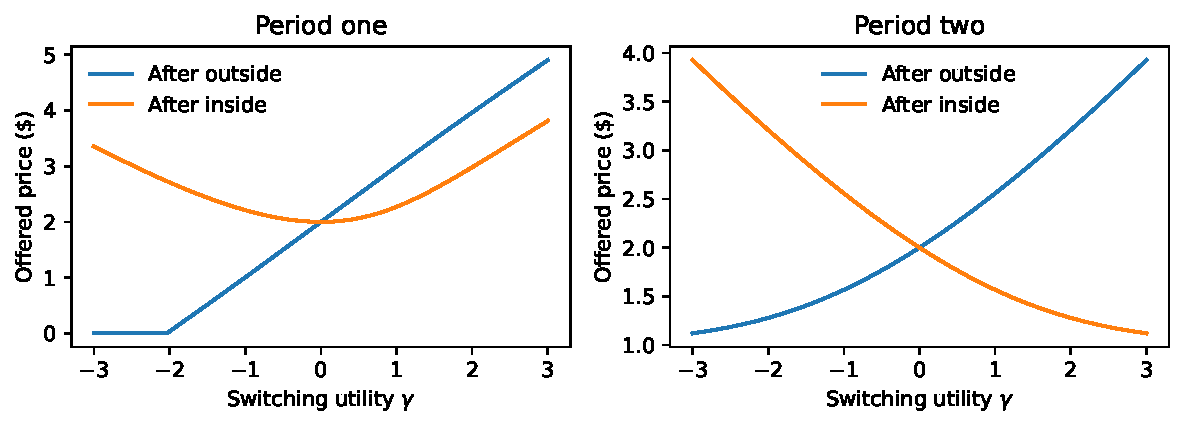
\includegraphics[width=.9\linewidth,height=.68\textheight,keepaspectratio]{assets/current/theory-prices.pdf}
\caption{Optimal prices by switching utility and previous choice.}
\label{fig:supply-prices}
\end{figure}
\begin{figure}[htbp]
\centering
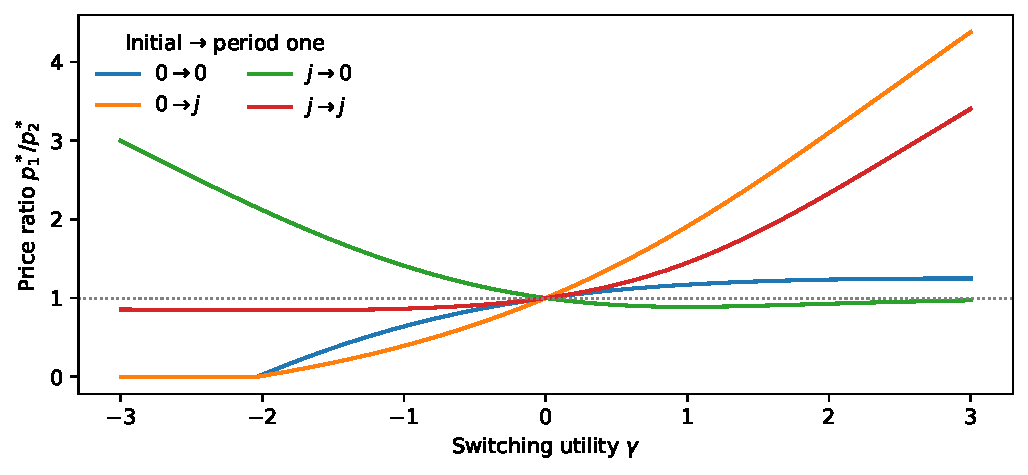
\includegraphics[width=.9\linewidth,height=.68\textheight,keepaspectratio]{assets/current/theory-ratios.pdf}
\caption{First-to-second-period price ratios by purchase history. The horizontal line marks equal prices.}
\label{fig:supply-history-ratios}
\end{figure}
\begin{figure}[htbp]
\centering
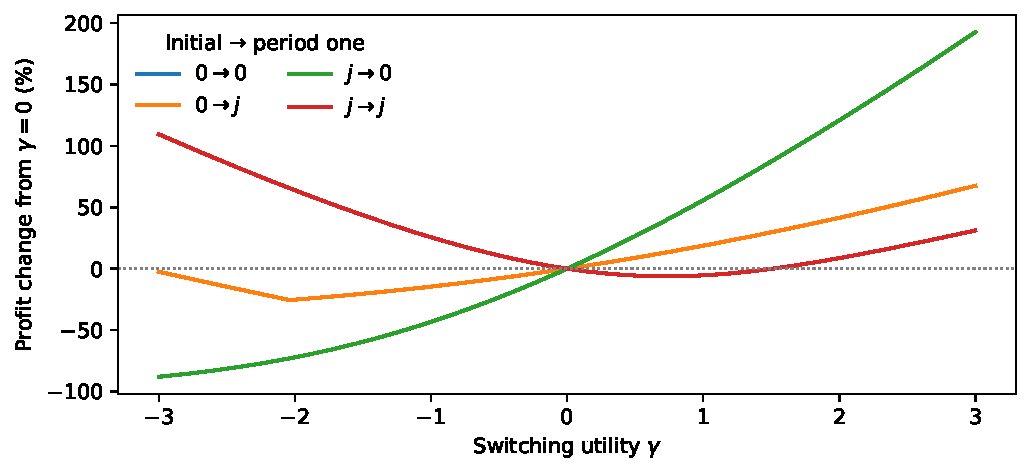
\includegraphics[width=.9\linewidth,height=.68\textheight,keepaspectratio]{assets/current/theory-history-profit.pdf}
\caption{Change in profit conditional on the initial state and period-one choice, relative to the same history at $\gamma=0$ (percent).}
\label{fig:supply-history-profit}
\end{figure}
\FloatBarrier

From \ref{fig:supply-history-profit}, we can see that the higher switching consumers are the most profitable on average. This is due to the switching utility overcoming the disutility of higher prices. For the low type, the habitually inside consumer is the second most profitable type. This is because they can be charged a high price in both periods with a low likelihood of switching to the outside good.

These figures show that switching type is meaningfully impactful on profits. Therefore, it is a natural extension to understand how valuable the information on types is to the firm.

\subsection{Uncertainty about Switching Type}

The firm now knows only the distribution of $\gamma$, but cannot observe individual consumers' types. They still observe purchase histories. Because the firm does not know exactly which consumers are which type, it assigns fixed probabilities to switching types:
\begin{equation}
 \gamma_r\in\{-2.5,-1.25,0,1.25,2.5\},\qquad
 \mu_r=\Pr(\gamma=\gamma_r),\qquad\sum_r\mu_r=1.
\end{equation}
Compare the equal prior $(1/5,1/5,1/5,1/5,1/5)$ and the five permutations of
$(0.50,0.1,0.1,0.1,0.1)$. All other parameters retain the numerical supply calibration.
The firm keeps the same beliefs in both periods and after either purchase outcome:
\begin{equation}
 \mu_{r,1}(h)=\mu_{r,2}(j)=\mu_{r,2}(0)=\mu_r.
\end{equation}
History changes demand and terminal prices, but does not change type probabilities.
The fixed-belief mixture demand is
\begin{equation}
 A(p,h;\mu)=\sum_r\mu_r
 \frac{e^{\beta+\alpha p+q(h)\gamma_r}}
 {1+e^{\beta+\alpha p+q(h)\gamma_r}}.
\end{equation}
Terminal values and the first-period objective are
\begin{align}
 \pi_2(a;\mu)&=\max_{x\geq 0} A(x,a;\mu)(x-c),\\
 \Pi^{\mathrm{fixed}}(h,\mu)&=\max_{p\geq 0}\bigl\{
 A(p,h;\mu)(p-c)\notag\\
 &\quad+[A(p,h;\mu)\pi_2(j;\mu)
 +(1-A(p,h;\mu))\pi_2(0;\mu)]\bigr\}.
\end{align}
The table compares this fixed-belief objective with prior-weighted known-type
profit. The reported difference is
\begin{equation}
 \mathcal I(h,\lambda)=\sum_r\lambda_r\Pi_r^*(h)
 -\Pi^{\mathrm{fixed}}(h,\lambda).
\end{equation}
%Derivations are in Appendix~\ref{app:gamma-uncertainty}.

\begin{figure}[htbp]
\centering
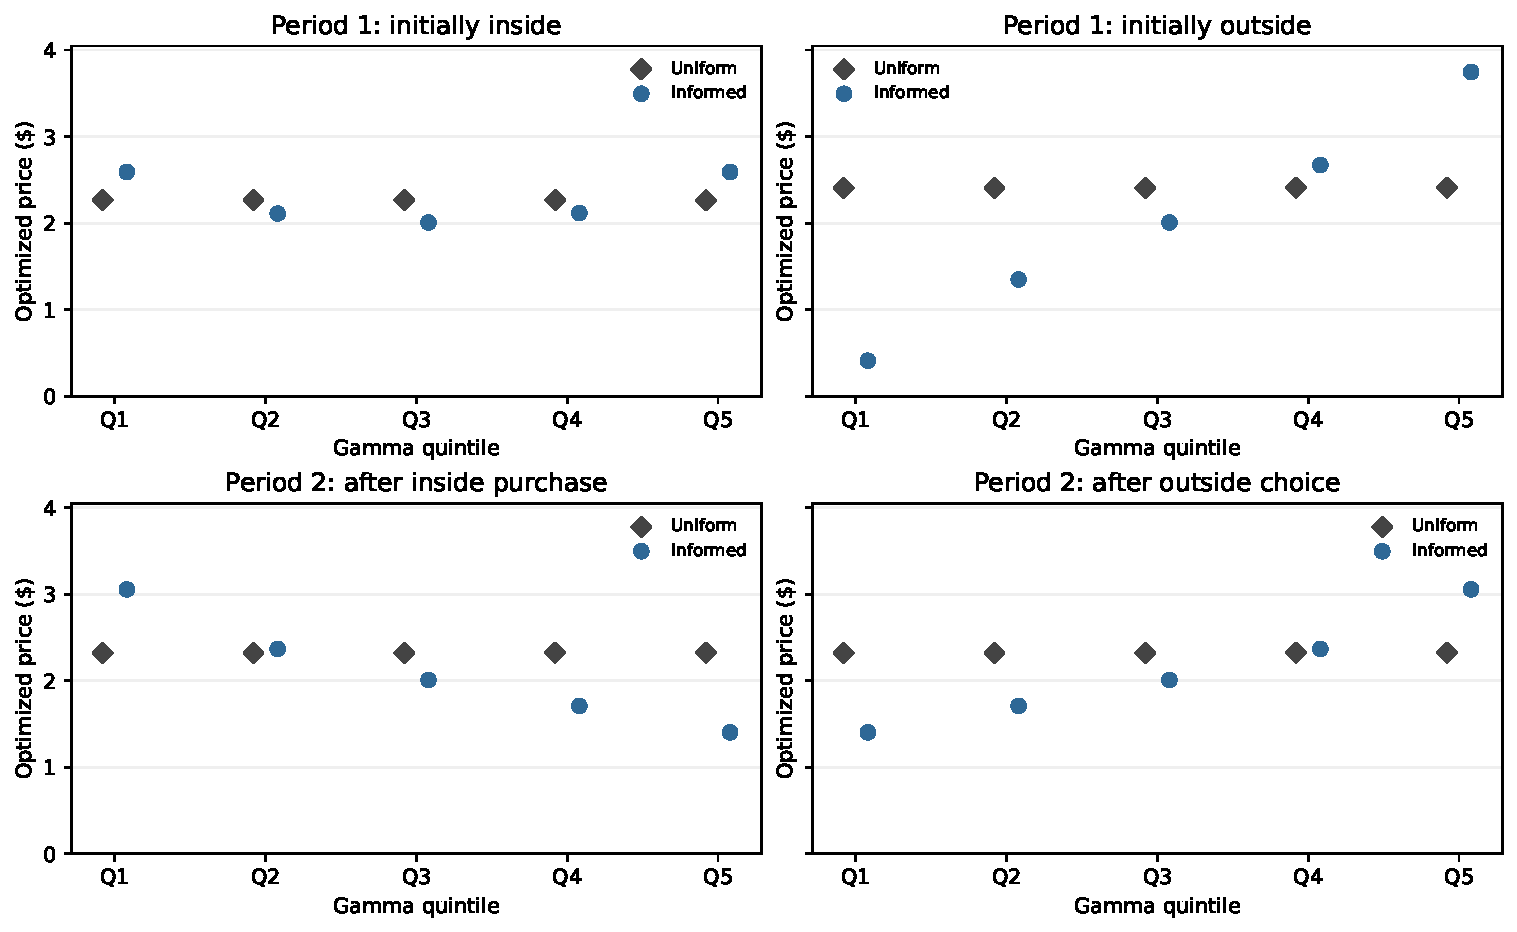
\includegraphics[width=\linewidth,height=.67\textheight,keepaspectratio]{assets/pricing_comparison/theory-prices.pdf}
\label{fig:theory-prices}
\end{figure}
\begin{figure}[htbp]
\centering
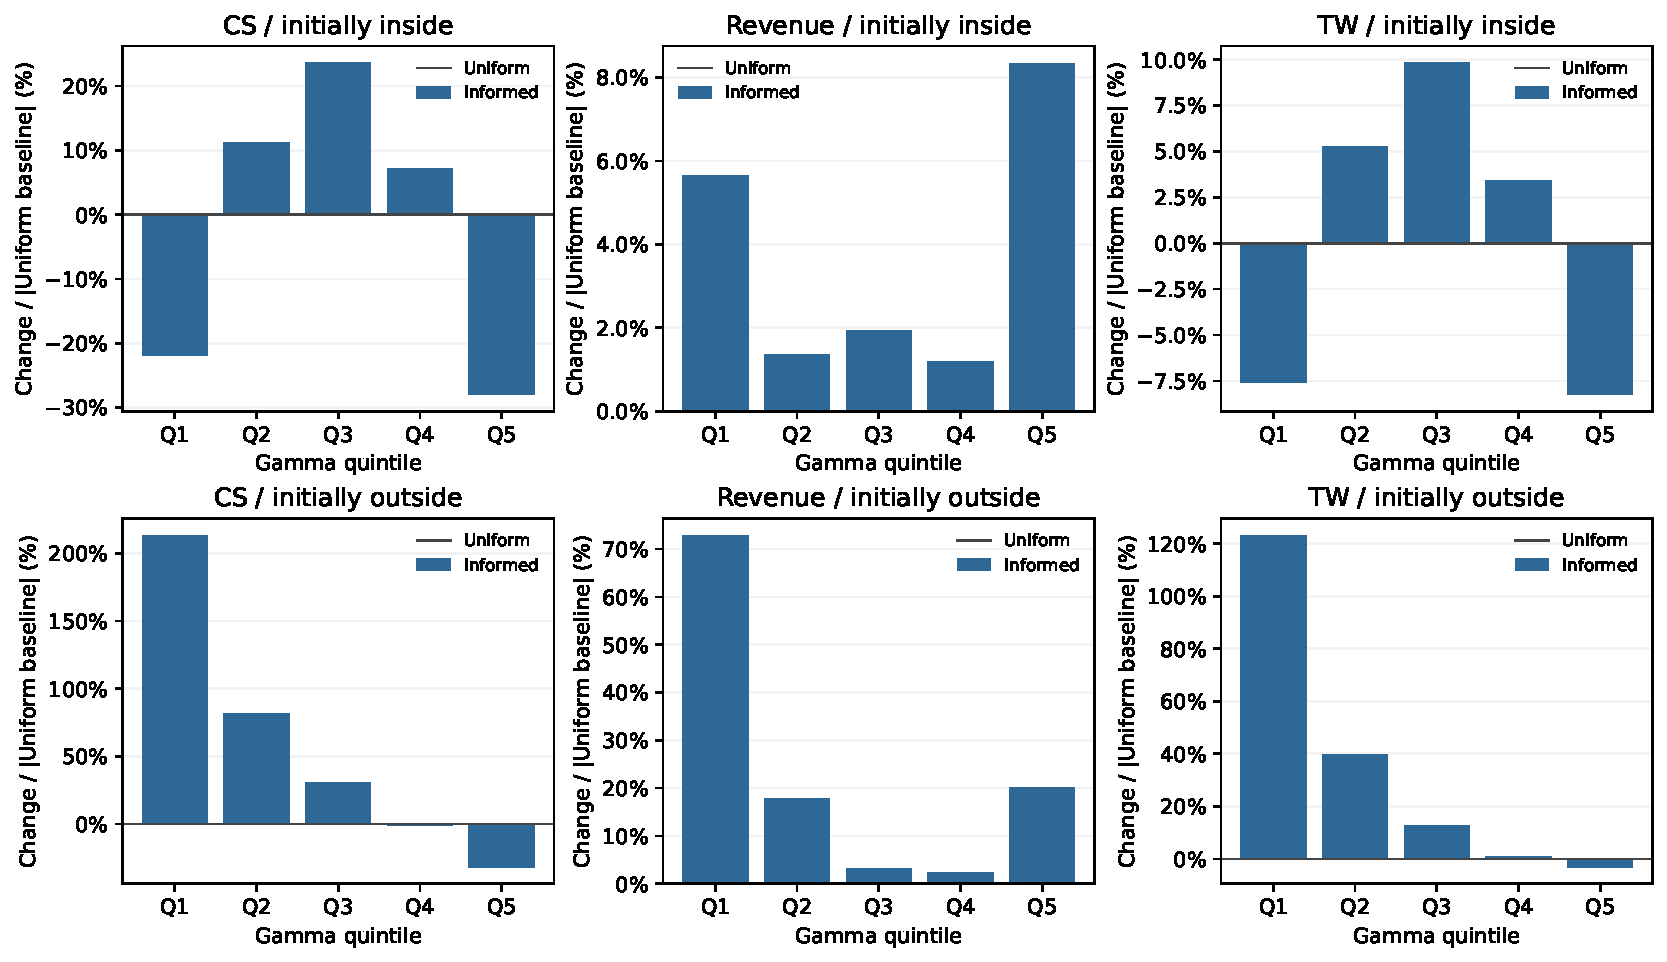
\includegraphics[width=\linewidth,height=.67\textheight,keepaspectratio]{assets/pricing_comparison/theory-welfare.pdf}
\label{fig:theory-welfare}
\end{figure}

Figure \ref{fig:theory-prices} shows that for the initially inside, known and uniform prices are relatively similar but the known price distribution still follows the convex shape presented in \ref{fig:supply-prices}. For the outside, we see the linearly increasing pattern in both periods. More interestingly, welfare analysis allows for understanding of which consumers are most impacted. It appears that the highest and lowest types of inside consumers are the worst off, with the firming able to capitalize the most on their type when known. For the outside consumers, The lowest type is best off due to the massive period one discount received under known pricing. Even after the increase in period two, this type of consumer still pays a lower price under targeted pricing than under uniform pricing. This is the best scenario for overall welfare, with the firm extracting greater revenue, though not at the expense of consumer surplus.

\section{Discussion of Theoretical Results}
\label{sec:theory-discussion}
% Author to write. Previous discussion is preserved in supply_previous.tex;
% its unconditional sign claims do not apply to the current model.

The theory presented in this section informs useful patterns to keep in mind. Firstly, initial purchase state is vital to the firm's pricing decision as well as profit. An initially outside consumer will require a large discount in period one in order to be able to capitalize on them in period two. An initially inside consumer will require strategic pricing in order to capitalize most effectively at a give price, with signage varying by switching type.

These illustrative results provide a framework with which we can understand how an empirical distribution of switching types will act. To do that, I first must estimate a demand system and then apply the estimated distribution to the supply model. 

% ============================================================
% EMPIRICAL DEMAND SIDE
% ============================================================

\section{Data}
\label{sec:data}

\subsection{Data Sources}



\subsection{Sample Construction}

\subsection{Variable Construction}

\subsection{Summary Statistics}
The no-habit flavor-switching estimation sample contains 15,752 households and 2,034,618 weeks.

%\input{assets/results/summary_statistics/full_panel_vs_yogurt.tex}
%\FloatBarrier
%\input{assets/results/summary_statistics/yogurt_dynamics.tex}
%\FloatBarrier
%\begin{figure}[htbp]
%\centering
%\includegraphics[width=\linewidth,height=.65\textheight,keepaspectratio]{assets/results/summary_statistics/flavor_hhi_histogram.pdf}
%\caption{Distribution of household flavor concentration}
%\label{fig:flavor-hhi}
%\end{figure}
%\FloatBarrier
%\begin{figure}[htbp]
%\centering
%\includegraphics[width=\linewidth,height=.65\textheight,keepaspectratio]{assets/results/summary_statistics/flavor_shares.pdf}
%\caption{Shares of purchased packages by detailed flavor}
%\label{fig:flavor-shares}
%\end{figure}
%\FloatBarrier
%\begin{figure}[htbp]
%\centering
%\includegraphics[width=\linewidth,height=.65\textheight,keepaspectratio]{assets/results/summary_statistics/aggregated_flavors/flavor_transitions.pdf}
%\caption{Transitions across aggregated flavor groups}
%\label{fig:flavor-transitions}
%\end{figure}
%\FloatBarrier

% ============================================================
% DEMAND MODEL
% ============================================================

\section{Demand Model}
\label{sec:demand-model}
The flavor-level specification below describes the demand model. The no-habit fit used in the plain-yogurt pricing exercise sets $\phi_i=0$ for all consumers.

\subsection{Choice Setting and Purchase History}
Let $i$ index consumers and $t$ calendar weeks. The inside alternatives are
\begin{equation*}
 \mathcal J=\{\mathrm{berry},\mathrm{plain},\mathrm{other}\}.
\end{equation*}
Alternative $0$ is the outside good. Let $y_{ijt}$ denote the number of packages
of flavor $j$ purchased in week $t$. For observed yogurt purchase weeks,
\begin{align}
 Q_{it}&=\sum_{j\in\mathcal J}y_{ijt},\\
 y_{i0t}&=\max\{0,7-Q_{it}\},\\
 M_{it}&=Q_{it}+y_{i0t}=\max\{7,Q_{it}\}.
\end{align}
Let $\mathcal H_i$ contain the observed purchase weeks used to construct history,
and $\mathcal T_i\subseteq\mathcal H_i$ the weeks retained for estimation.
The share of each inside flavor in a purchase week is
\begin{equation}
 w_{ijt}=\frac{y_{ijt}}{Q_{it}},\qquad t\in\mathcal H_i.
\end{equation}
Novelty is the share of other flavors purchased in the immediately preceding
calendar week:
\begin{equation}
 N_{ijt}=\begin{cases}
 \displaystyle\sum_{k\in\mathcal J,\,k\ne j}w_{ik,t-1}=1-w_{ij,t-1},
 &t-1\in\mathcal H_i,\\[3pt]
 0,&t-1\notin\mathcal H_i.
 \end{cases}
 \label{eq:empirical-novelty}
\end{equation}
Since $0\le w_{ij,t-1}\le1$, novelty satisfies $N_{ijt}\in[0,1]$.
It equals one when last week's basket contained other flavors and no $j$, and
zero when the basket contained only $j$.

For example, suppose last week a consumer bought three berry packages and one
plain package. The novelty of each possible flavor choice this week is
\begin{equation}
 \begin{aligned}
 N_{i,\mathrm{berry},t}&=1-\frac{3}{4}=0.25,\\
 N_{i,\mathrm{plain},t}&=1-\frac{1}{4}=0.75,\\
 N_{i,\mathrm{other},t}&=1-\frac{0}{4}=1.
 \end{aligned}
 \label{eq:novelty-example}
\end{equation}
Choosing berry differs from one quarter of last week's purchases; choosing
plain differs from three quarters; choosing other differs from all of them.
Thus $N_{ijt}$ measures switching intensity relative to the previous basket
for a possible choice of $j$, rather than the realized change in the entire
basket. Its contribution to utility is $\gamma_iN_{ijt}$: positive $\gamma_i$
rewards novelty, while negative $\gamma_i$ penalizes it.


The habit measure in the fitted model is cumulative own-flavor stock:
\begin{equation}
 H_{ijt}=\sum_{\substack{s\in\mathcal H_i\\s<t}}w_{ijs}.
 \label{eq:empirical-habit}
\end{equation}
Both histories start at zero. Missing purchase weeks contribute no stock and
set the next week's novelty measure to zero; they are not inserted as outside-choice weeks.

\subsection{Utility and Consumer Heterogeneity}
\begin{align}
 U_{ijt}&=V_{ijt}+\varepsilon_{ijt},\\
 V_{ijt}&=\beta_0+\beta_j+\gamma_iN_{ijt}+\phi_iH_{ijt}+\alpha_i p_{ijt},
 \qquad j\in\mathcal J,
 \label{eq:utility}\\
 U_{i0t}&=\varepsilon_{i0t},\qquad V_{i0t}=0.
\end{align}
The flavor constants are relative to other: $\beta_{\mathrm{other}}=0$.
The shocks are independent unit-scale Type-I extreme value.
The three random coefficients are fixed within consumer:
\begin{align}
 \alpha_i&=-\exp(\mu_\alpha+\sigma_\alpha\nu_{i\alpha}),\\
 \gamma_i&=\mu_\gamma+\sigma_\gamma\nu_{i\gamma},\\
 \phi_i&=\mu_\phi+\sigma_\phi\nu_{i\phi},\\
 \nu_i&=(\nu_{i\alpha},\nu_{i\gamma},\nu_{i\phi})'
 \sim\mathcal N(0,I_3).
\end{align}
Thus $\alpha_i<0$, while novelty and habit coefficients are unrestricted in sign.

\subsection{Choice Probabilities and Market Shares}
Let $\mathcal A_{it}\subseteq\mathcal J$ denote the flavors available at the
consumer's exposure store, and $\mathcal A_{it}^0=\mathcal A_{it}\cup\{0\}$.
Conditional on the consumer's type,
\begin{align}
 P_{ijt}(\nu_i;\theta)
 &=\frac{\exp\{V_{ijt}(\nu_i;\theta)\}}
 {1+\sum_{k\in\mathcal A_{it}}\exp\{V_{ikt}(\nu_i;\theta)\}},
 \qquad j\in\mathcal A_{it},
 \label{eq:choice-probability}\\
 P_{i0t}(\nu_i;\theta)
 &=\frac{1}{1+\sum_{k\in\mathcal A_{it}}\exp\{V_{ikt}(\nu_i;\theta)\}}.
\end{align}
Unavailable inside alternatives have zero probability.
Integrate over types before averaging across consumers:
\begin{align}
 \overline P_{ijt}(\theta)
 &=\int P_{ijt}(\nu;\theta)\varphi_3(\nu)\,d\nu,\\
 s_{jt}(\theta)&=\frac{1}{N_t}\sum_{i:\,t\in\mathcal T_i}\overline P_{ijt}(\theta).
\end{align}
Here $N_t$ is the number of retained consumers in week $t$.

\section{Estimation}
The plain-yogurt calibration uses the no-habit variant of the flavor-level estimator.
\label{sec:estimation}

\subsection{Identification}
\label{subsec:identification}
% Author to write: identifying variation, price exogeneity in the no-control
% specification, and conditioning on observed initial histories.

\subsection{Simulated Maximum Likelihood}
\label{subsec:estimation-procedure}
Conditional on a persistent consumer type, the panel likelihood is
\begin{equation}
 L_i(\nu;\theta)=\prod_{t\in\mathcal T_i}
 \prod_{j\in\mathcal A_{it}^0}P_{ijt}(\nu;\theta)^{y_{ijt}}.
\end{equation}
Integrating over types gives
\begin{equation}
 L_i(\theta)=\int L_i(\nu;\theta)\varphi_3(\nu)\,d\nu.
\end{equation}
Use $R=128$ standard normal draws per consumer, held fixed across weeks and
objective evaluations:
\begin{align}
 \widehat L_i(\theta)&=\frac{1}{128}\sum_{r=1}^{128}
 \prod_{t\in\mathcal T_i}\prod_{j\in\mathcal A_{it}^0}
 P_{ijt}(\nu_{ir};\theta)^{y_{ijt}},\\
 Q_{128}(\theta)&=-\sum_{i=1}^N\log\widehat L_i(\theta),
 \label{eq:estimation-objective}\\
 \widehat\theta&=\argmin_\theta Q_{128}(\theta).
\end{align}
Multinomial count constants do not depend on $\theta$ and are omitted.
Run three optimization starts and retain the solution with the lowest objective.


\subsection{Inference}

% Author to write.

\subsection{No-Habit Flavor-Switching Fit}
The fit sets $\phi_i=0$ and integrates over the remaining two persistent
coefficients using 128 antithetic normal draws. It estimates fixed flavor
intercepts, normally distributed switching utility, and lognormally
distributed absolute price sensitivity. The fit omits the price control function.

% ============================================================
% EMPIRICAL RESULTS
% ============================================================

\section{Results}
\label{sec:results}

\subsection{Demand Estimates}
\begin{table}[htbp]
\centering\small
\caption{No-habit flavor-switching demand estimates used to calibrate plain-yogurt pricing.}
\label{tab:demand-estimates}
\begin{tabular}{lrr}
\toprule
Parameter & Estimate & Std. error \\
\midrule
Inside constant (other yogurt) & 0.0162 & 0.0026 \\
Berry increment & -1.6356 & 0.0027 \\
Plain increment & -1.3013 & 0.0038 \\
Mean of $\log(-\alpha_i)$ & 0.4834 & 0.0039 \\
Mean of switching utility $\gamma_i$ & -0.8382 & 0.0145 \\
SD of switching utility $\gamma_i$ & 2.0992 & 0.0140 \\
SD of $\log(-\alpha_i)$ & 1.2474 & 0.0047 \\
\bottomrule
\end{tabular}
\end{table}


%\input{assets/results/demand/estimates.tex}
%\FloatBarrier
%\input{assets/results/demand/comparison.tex}
%\FloatBarrier

\subsection{Price Elasticities}
At a given history, the conditional own-price elasticity of plain-yogurt
demand in the pricing exercise is $\alpha p[1-s(p,h;\gamma)]$.

\subsection{State Dependence}
The fitted mean switching coefficient is $-0.8382$, with a standard
deviation of $2.0992$.

\subsection{Consumer Heterogeneity}
Figure~\ref{fig:trimmed-distribution} shows the fitted distribution of
switching utility and the five quintiles of the retained distribution used
in the plain-yogurt pricing exercise.

\begin{figure}[htbp]
\centering
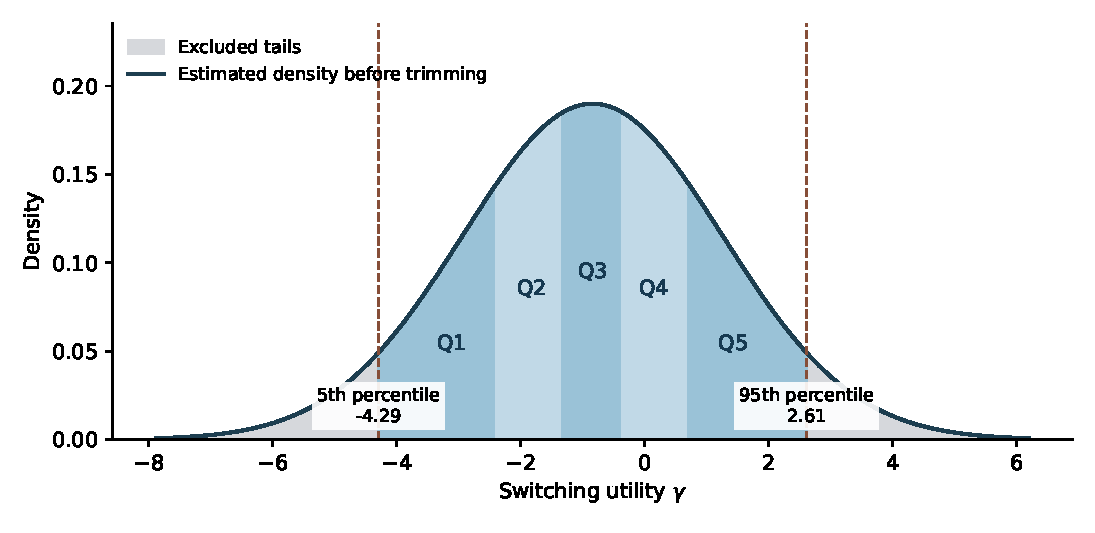
\includegraphics[width=\linewidth,height=.67\textheight,keepaspectratio]{assets/pricing_comparison/trimmed-distribution.pdf}
\caption{Fitted switching-utility distribution before trimming. Shading between the dashed cutoff lines identifies the five quintiles used for pricing.}
\label{fig:trimmed-distribution}
\end{figure}

\FloatBarrier

%\begin{figure}[htbp]
%\centering
%\includegraphics[width=\linewidth,height=.65\textheight,keepaspectratio]{assets/results/demand/history_distributions.pdf}
%\caption{Estimated distributions of novelty and habit coefficients}
%\label{fig:history-distributions}
%\end{figure}
%\FloatBarrier

% ============================================================
% ROBUSTNESS
% ============================================================
%
%\section{Robustness}
%\label{sec:robustness}
%
%\subsection{Alternative Specifications}
%
%\subsection{Alternative Samples}
%
%\subsection{Alternative Definitions}


% ============================================================
% DISCUSSION OF EMPIRICAL RESULTS
% ============================================================

\section{Discussion of Empirical Results}
\label{sec:empirical-discussion}

\subsection{Economic Magnitudes}

%\input{assets/results/demand/implied_wtp.tex}
%\FloatBarrier

\subsection{Relationship to Theoretical Predictions}

\subsection{Economic Interpretation}


% ============================================================
% SUPPLY-DEMAND CONNECTION
% ============================================================

\section{Connecting Demand Estimates to Firm Pricing}
\label{sec:supply-demand}

\subsection{Estimated Demand and Optimal Prices}
Plain yogurt is the inside good. Berry yogurt, other yogurt, and no yogurt
make up the outside option. Pricing holds the plain intercept at
$\beta=-1.2851$ and the mean price coefficient at $\alpha=-3.5304$.
The pricing distribution is the estimated normal switching distribution
trimmed at the 5th and 95th percentiles and renormalized. The five pricing
quintiles each contain one fifth of the retained distribution. The firm
chooses nonnegative offers with zero marginal cost and no discounting.

%
%\subsubsection{Berry}
%\begin{figure}[htbp]
%\centering
%\includegraphics[width=\linewidth,height=.65\textheight,keepaspectratio]{assets/results/pricing/berry/household_coupon_results.pdf}
%\caption{Berry: consumer types and expected revenue}
%\label{fig:revenue-berry}
%\end{figure}
%\FloatBarrier
%\begin{figure}[htbp]
%\centering
%\includegraphics[width=\linewidth,height=.65\textheight,keepaspectratio]{assets/results/pricing/berry/discounts_by_consumer_type.pdf}
%\caption{Berry: optimal offers by consumer type}
%\label{fig:offers-berry}
%\end{figure}
%\FloatBarrier
%\subsubsection{Plain}
%\begin{figure}[htbp]
%\centering
%\includegraphics[width=\linewidth,height=.65\textheight,keepaspectratio]{assets/results/pricing/plain/household_coupon_results.pdf}
%\caption{Plain: consumer types and expected revenue}
%\label{fig:revenue-plain}
%\end{figure}
%\FloatBarrier
%\begin{figure}[htbp]
%\centering
%\includegraphics[width=\linewidth,height=.65\textheight,keepaspectratio]{assets/results/pricing/plain/discounts_by_consumer_type.pdf}
%\caption{Plain: optimal offers by consumer type}
%\label{fig:offers-plain}
%\end{figure}
%\FloatBarrier

\subsection{Counterfactual Pricing}
Figure~\ref{fig:plain-prices} reports the optimized offers for plain yogurt
by purchase history under the uniform and quintile-informed policies.

%\begin{figure}[htbp]
%\centering
%\includegraphics[width=\linewidth,height=.65\textheight,keepaspectratio]{assets/results/pricing/berry/pricing_mechanism.pdf}
%\caption{Berry: price paths}
%\label{fig:mechanism-berry}
%\end{figure}
%\FloatBarrier
%\begin{figure}[htbp]
%\centering
%\includegraphics[width=\linewidth,height=.65\textheight,keepaspectratio]{assets/results/pricing/plain/pricing_mechanism.pdf}
%\caption{Plain: price paths}
%\label{fig:mechanism-plain}
%\end{figure}
%\FloatBarrier

%\input{assets/results/pricing/benchmarks.tex}
%\FloatBarrier
%\begin{figure}[htbp]
%\centering
%\includegraphics[width=\linewidth,height=.65\textheight,keepaspectratio]{assets/results/pricing/plain/pricing_policy_benchmarks.pdf}
%\caption{Plain: no-coupon, common-coupon, and personalized pricing benchmarks.}
%\label{fig:benchmarks-plain}
%\end{figure}
%\FloatBarrier
%\begin{figure}[htbp]
%\centering
%\includegraphics[width=\linewidth,height=.65\textheight,keepaspectratio]{assets/results/pricing/plain/terminal_offers_by_purchase.pdf}
%\caption{Plain: price paths under common and personalized pricing.}
%\label{fig:terminal-conditional-plain}
%\end{figure}
%\FloatBarrier
%\begin{figure}[htbp]
%\centering
%\includegraphics[width=\linewidth,height=.65\textheight,keepaspectratio]{assets/results/pricing/berry/pricing_policy_benchmarks.pdf}
%\caption{Berry: no-coupon, common-coupon, and personalized pricing benchmarks.}
%\label{fig:benchmarks-berry}
%\end{figure}
%\FloatBarrier
%\begin{figure}[htbp]
%\centering
%\includegraphics[width=\linewidth,height=.65\textheight,keepaspectratio]{assets/results/pricing/berry/terminal_offers_by_purchase.pdf}
%\caption{Berry: price paths under common and personalized pricing.}
%\label{fig:terminal-conditional-berry}
%\end{figure}
%\FloatBarrier
%
%\subsection{Counterfactual Outcomes}
%
%\input{assets/results/pricing/focal_flavor_comparison.tex}
%\FloatBarrier
%

% ============================================================
% COUNTERFACTUALS AND WELFARE
% ============================================================

\subsection{Empirical Information Friction}
\label{subsec:empirical-information}
The uniform firm observes whether the consumer previously chose plain
yogurt and uses the full trimmed distribution of $\gamma$. The informed
counterfactual also reveals the consumer's quintile. The same population
distribution applies to both initial histories, and neither policy updates
its type weights after a choice. The comparison conditions on initial history.

%\begin{figure}[htbp]
%\centering
%\includegraphics[width=\linewidth,height=.65\textheight,keepaspectratio]{assets/results/empirical_information/plain/revenues.pdf}
%\caption{Plain: known-type and fixed-belief policies evaluated under persistent consumer types.}
%\label{fig:empirical-information-revenues-plain}
%\end{figure}
%\FloatBarrier
%\begin{figure}[htbp]
%\centering
%\includegraphics[width=\linewidth,height=.65\textheight,keepaspectratio]{assets/results/empirical_information/plain/information_value.pdf}
%\caption{Plain: revenue gain from observing novelty type under a common persistent-type evaluation.}
%\label{fig:empirical-information-value-plain}
%\end{figure}
%\FloatBarrier
%\begin{figure}[htbp]
%\centering
%\includegraphics[width=\linewidth,height=.65\textheight,keepaspectratio]{assets/results/empirical_information/berry/revenues.pdf}
%\caption{Berry: known-type and fixed-belief policies evaluated under persistent consumer types.}
%\label{fig:empirical-information-revenues-berry}
%\end{figure}
%\FloatBarrier
%\begin{figure}[htbp]
%\centering
%\includegraphics[width=\linewidth,height=.65\textheight,keepaspectratio]{assets/results/empirical_information/berry/information_value.pdf}
%\caption{Berry: revenue gain from observing novelty type under a common persistent-type evaluation.}
%\label{fig:empirical-information-value-berry}
%\end{figure}
%\FloatBarrier

\section{Counterfactuals and Welfare}
\label{sec:counterfactuals}

\subsection{Counterfactual Experiments}
We compare uniform and quintile-informed pricing for plain yogurt.
Percentage changes are $100(X_{\mathrm{Informed}}-X_{\mathrm{Uniform}})/|X_{\mathrm{Uniform}}|$.
A zero Uniform baseline yields an undefined percentage change.

\begin{figure}[htbp]
\centering
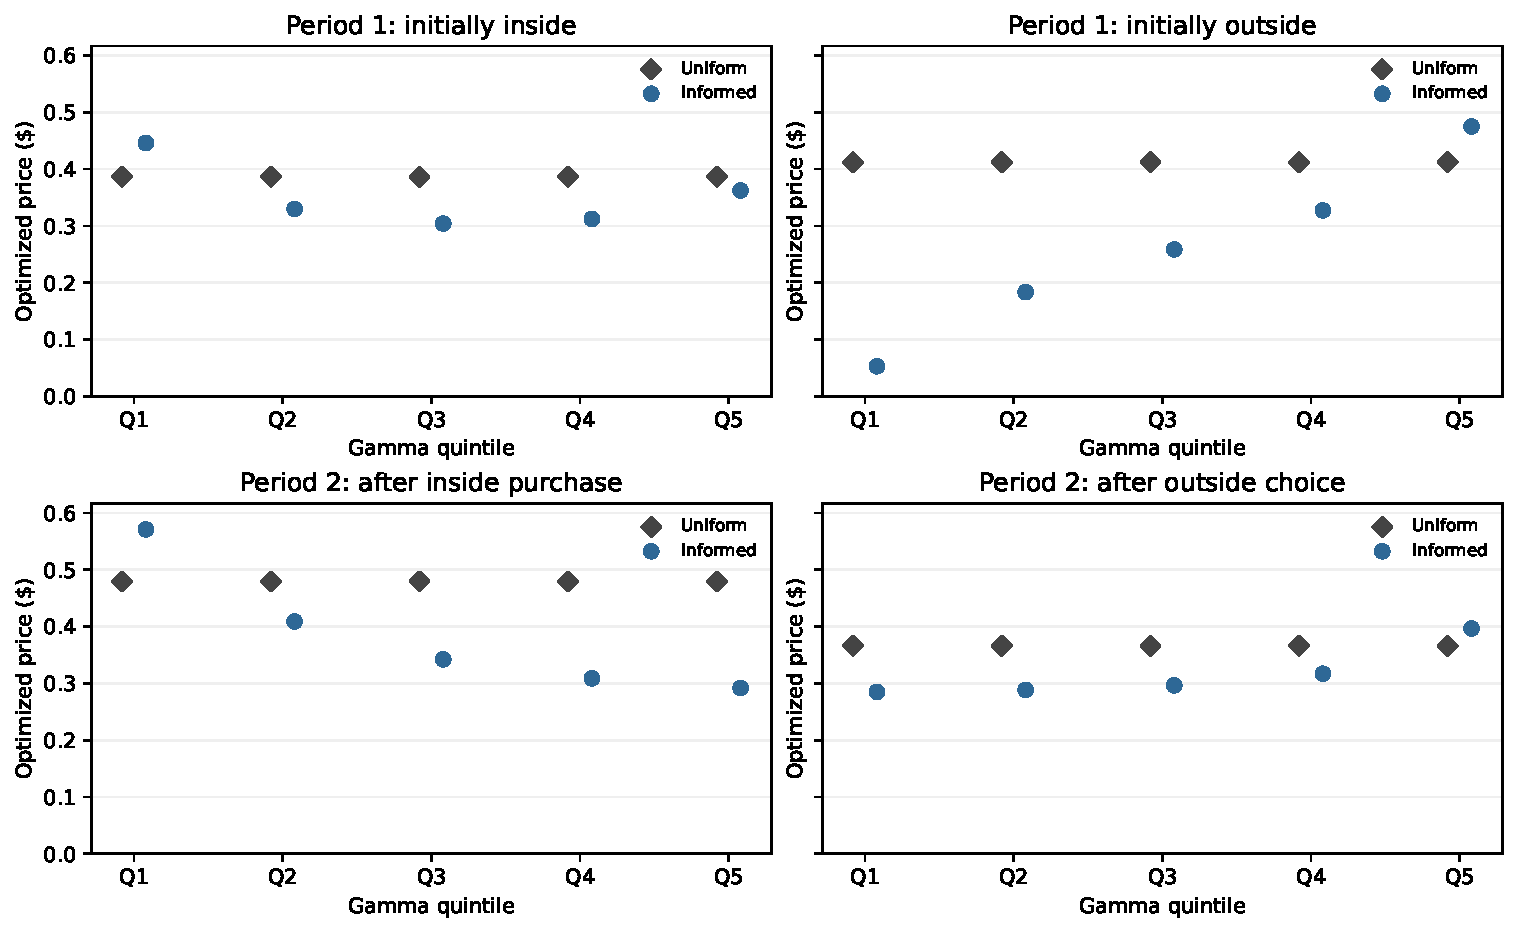
\includegraphics[width=\linewidth,height=.67\textheight,keepaspectratio]{assets/pricing_comparison/plain-prices.pdf}
\caption{Plain-yogurt offers with nonnegative prices. Uniform offers are the same across quintiles at a given history.}
\label{fig:plain-prices}
\end{figure}
\begin{figure}[htbp]
\centering
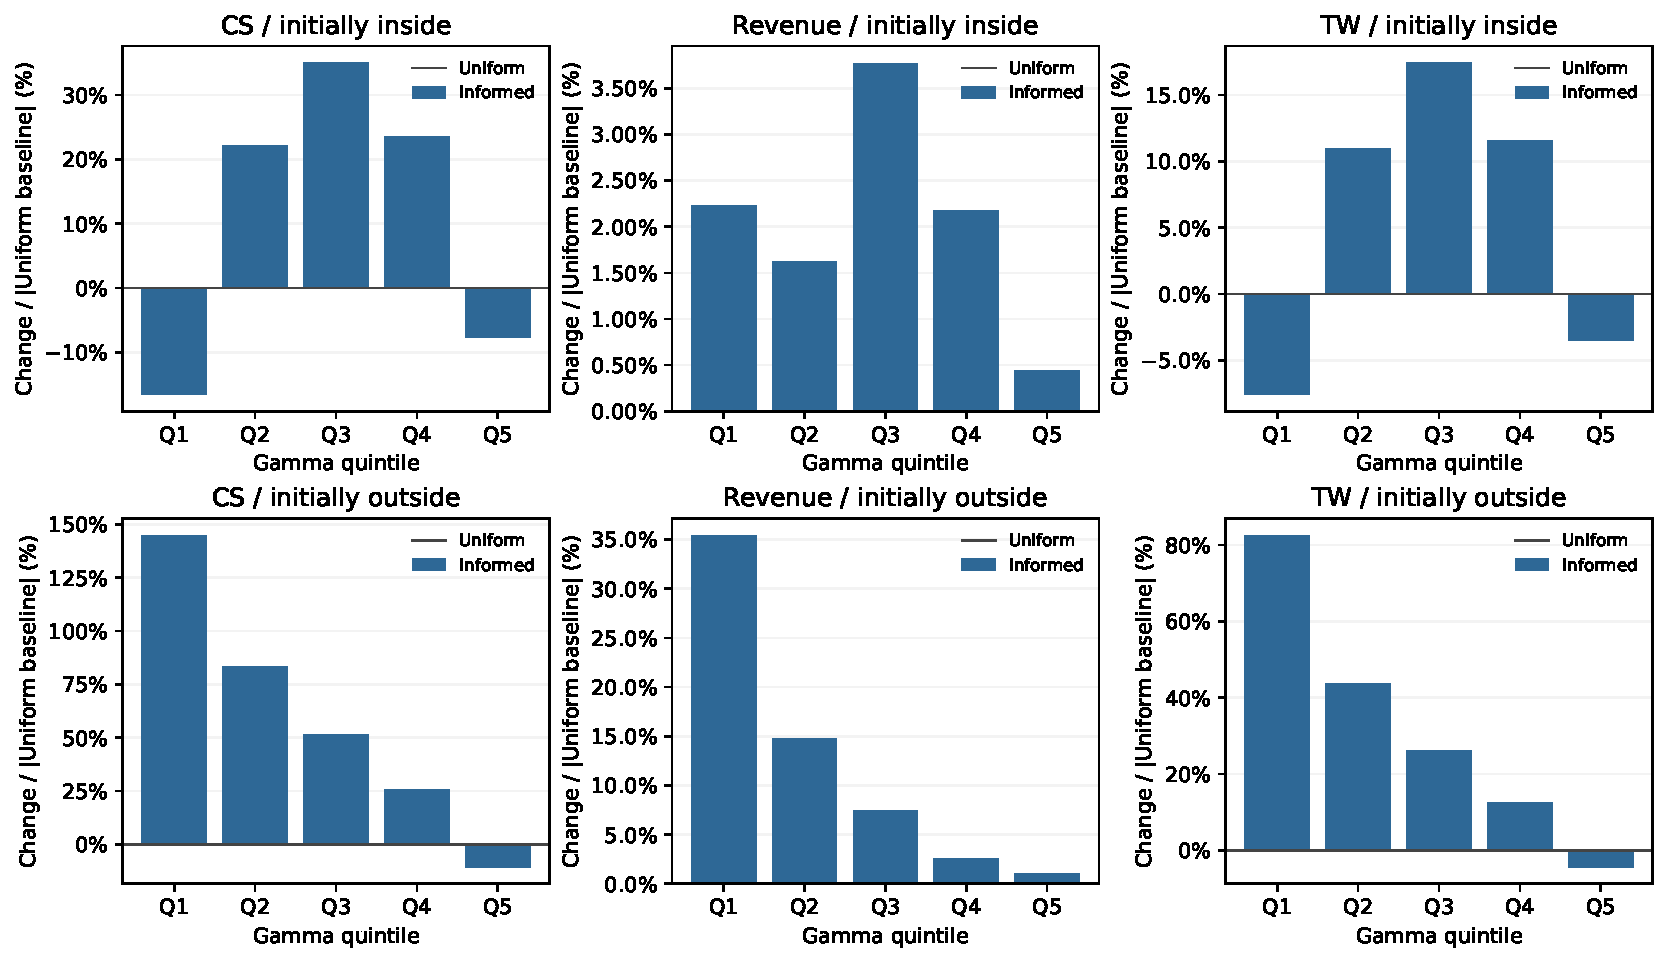
\includegraphics[width=\linewidth,height=.67\textheight,keepaspectratio]{assets/pricing_comparison/plain-welfare.pdf}
\caption{Plain-yogurt welfare and revenue changes by initial state and quintile (percent relative to the absolute Uniform baseline).}
\label{fig:plain-welfare}
\end{figure}
\begin{table}[htbp]
\centering\small
\caption{Welfare and revenue by initial state, averaging levels over quintiles. Levels are dollars per consumer over two periods. Changes are relative to Uniform.}
\label{tab:plain-averages}
\begin{tabular}{llrrr}
\toprule
Initial state & Outcome & Uniform & Informed & Change (\%) \\
\midrule
Outside & Consumer surplus & 0.0436 & 0.0467 & +6.95 \\
Outside & Revenue & 0.0535 & 0.0551 & +2.96 \\
Outside & Total welfare & 0.0971 & 0.1018 & +4.75 \\
Inside & Consumer surplus & 0.1549 & 0.1507 & -2.75 \\
Inside & Revenue & 0.1602 & 0.1634 & +2.01 \\
Inside & Total welfare & 0.3151 & 0.3141 & -0.33 \\
\bottomrule
\end{tabular}
\end{table}


\subsection{Consumer Surplus}
Consumer surplus sums the expected log-sum surplus relative to the outside
option at each history over the two periods. Averaging over quintiles,
consumer surplus rises by 6.95\% for consumers who start outside and falls
by 2.75\% for consumers who start inside.

\subsection{Firm Profits}
With zero marginal cost, revenue equals profit. Averaging over quintiles,
revenue rises by 2.96\% for consumers who start outside and by 2.01\% for
consumers who start inside.

\subsection{Total Welfare}
Total welfare rises by 4.75\% for consumers who start outside and falls by
0.33\% for consumers who start inside, averaging over quintiles.

% ============================================================
% CONCLUSION
% ============================================================

\section{Conclusion}
\label{sec:conclusion}


% ============================================================
% REFERENCES
% ============================================================

\bibliographystyle{aer}
\bibliography{references}


% ============================================================
% APPENDIX
% ============================================================

\newpage
\appendix

\section{Supply-Side Derivations}
\label{app:supply}
\allowdisplaybreaks[1]

\subsection{Normalization and Demand Derivatives}
Subtracting outside deterministic utility gives
\begin{align}
 v_t(b)&=\beta+\alpha p_t(b)
 +\gamma\bigl[\mathbf{1}\{b=0\}-\mathbf{1}\{b=j\}\bigr]
 =\beta+\alpha p_t(b)+q(b)\gamma,\\
 \frac{\partial s_t}{\partial v_t}&=\frac{e^{v_t}}{(1+e^{v_t})^2}
 =s_t(1-s_t),\\
 ds_t&=s_t(1-s_t)[d\beta+p_t\,d\alpha+\alpha\,dp_t+q(b)\,d\gamma].
 \label{eq:supply-total-share}
\end{align}
The price and switching derivatives, holding history fixed, are
\begin{align}
 \frac{\partial s_t(h)}{\partial p_t(h)}&=\alpha s_t(h)s_{0t}(h),\\
 \left.\frac{\partial s_t(h)}{\partial\gamma}\right|_{p_t(h)}
 &=q(h)s_t(h)s_{0t}(h).
\end{align}
Multiplying the price derivatives by price and dividing by the corresponding
share gives the elasticities:
\begin{align}
 \epsilon_{jj,t}(h)&=\frac{p_t(h)}{s_t(h)}
 \frac{\partial s_t(h)}{\partial p_t(h)}
 =\alpha p_t(h)s_{0t}(h),\\
 \epsilon_{0j,t}(h)&=\frac{p_t(h)}{s_{0t}(h)}
 \frac{\partial s_{0t}(h)}{\partial p_t(h)}
 =-\alpha p_t(h)s_t(h).
\end{align}

\subsection{Backward Induction}
For either terminal state $a$,
\begin{align}
 \frac{d}{dp_2}\{s_2(p_2-c)\}
 &=s_2+\alpha s_2(1-s_2)(p_2-c)=0,\\
 1+\alpha(1-s_2^*)(p_2^*-c)&=0,\\
 p_2^*(a)-c&=-\frac{1}{\alpha[1-s_2^*(a)]},\\
 W_2(a)&=s_2^*(a)[p_2^*(a)-c]
 =-\frac{s_2^*(a)}{\alpha[1-s_2^*(a)]}.
\end{align}
Both continuation states enter first-period expected profit:
\begin{align}
 \Pi(p_1;h)&=s_1(p_1-c)+\delta[s_1W_2(j)+(1-s_1)W_2(0)]\\
 &=\delta W_2(0)+s_1[p_1-c+\delta\Delta W],\\
 \partial_{p_1}\Pi
 &=s_1+\alpha s_1(1-s_1)[p_1-c+\delta\Delta W],\\
 p_1^*-c+\delta\Delta W&=-\frac{1}{\alpha\ell},\\
 \Pi^*(h)&=\delta W_2(0)-\frac{s}{\alpha\ell}.
\end{align}

\subsection{Unique Global Optima}
Each pricing problem, up to an additive constant, has the form
\begin{equation}
 f(p)=s(p)(p-k),\quad s(p)=\frac{e^{b+\alpha p}}{1+e^{b+\alpha p}},
 \quad k=c\ \text{or}\ k=c-\delta\Delta W.
\end{equation}
\begin{align}
 f'(p)&=\frac{s(p)}{1+e^{b+\alpha p}}H(p),\\
 H(p)&=1+e^{b+\alpha p}+\alpha(p-k),\\
 H'(p)&=\alpha[1+e^{b+\alpha p}]<0,\\
 \lim_{p\to-\infty}H(p)&=+\infty,\qquad
 \lim_{p\to+\infty}H(p)=-\infty.
\end{align}
Thus $f'$ changes from positive to negative at a unique finite price,
which is the global maximizer. The first-period optimum can be below $c$.

\subsection{General Implicit and Envelope Derivatives}
For $\theta\in\{\gamma,\beta,\alpha,\delta\}$, define direct utility responses
\begin{align}
 D_{1\theta}&=\mathbf{1}\{\theta=\beta\}
 +p_1^*\mathbf{1}\{\theta=\alpha\}+q(h)\mathbf{1}\{\theta=\gamma\},\\
 D_{2\theta}(a)&=\mathbf{1}\{\theta=\beta\}
 +p_2^*(a)\mathbf{1}\{\theta=\alpha\}+q(a)\mathbf{1}\{\theta=\gamma\}.
\end{align}
The terminal envelope theorem and first-order condition imply
\begin{align}
 W_{2,\theta}(a)
 &=s_2^*(a)[1-s_2^*(a)]D_{2\theta}(a)[p_2^*(a)-c]
 =-\frac{s_2^*(a)D_{2\theta}(a)}{\alpha},\\
 0&=\frac{dp_2^*(a)}{d\theta}
 -\frac{\mathbf{1}\{\theta=\alpha\}}{\alpha^2[1-s_2^*(a)]}
 +\frac{ds_2^*(a)/d\theta}{\alpha[1-s_2^*(a)]^2},\\
 \frac{ds_2^*(a)}{d\theta}
 &=s_2^*(a)[1-s_2^*(a)]\left[D_{2\theta}(a)
 +\alpha\frac{dp_2^*(a)}{d\theta}\right],\\
 \frac{dp_2^*(a)}{d\theta}
 &=\frac{\mathbf{1}\{\theta=\alpha\}}{\alpha^2}
 -\frac{s_2^*(a)D_{2\theta}(a)}{\alpha}.
\end{align}
For the first-period pricing equation,
\begin{align}
 F&=p_1-c+\frac{1}{\alpha(1-s_1)}+\delta\Delta W=0,\\
 F_{p_1}&=1+\frac{s}{\ell}=\frac{1}{\ell},\\
 F_\theta&=-\frac{\mathbf{1}\{\theta=\alpha\}}{\alpha^2\ell}
 +\frac{sD_{1\theta}}{\alpha\ell}
 +\mathbf{1}\{\theta=\delta\}\Delta W+\delta\Delta W_\theta,\\
 \frac{dp_1^*}{d\theta}&=-\frac{F_\theta}{F_{p_1}}
 =\frac{\mathbf{1}\{\theta=\alpha\}}{\alpha^2}
 -\frac{sD_{1\theta}}{\alpha}
 -\ell[\mathbf{1}\{\theta=\delta\}\Delta W+\delta\Delta W_\theta].
 \label{eq:supply-general-derivative}
\end{align}
The continuation-value differences needed here are
\begin{align}
 \Delta W_\gamma&=(u+v)/\alpha,\\
 \Delta W_\beta&=(v-u)/\alpha,\\
 \Delta W_\alpha&=[vp_2^*(0)-up_2^*(j)]/\alpha,\\
 \Delta W_\delta&=0.
\end{align}
Substitution into \eqref{eq:supply-general-derivative} gives all four
first-period comparative statics in the text. In particular,
\begin{equation}
 W_2(j)\big|_{\gamma=0}=W_2(0)\big|_{\gamma=0},\qquad
 \Delta W_\gamma=B/\alpha<0
 \ \Longrightarrow\ \operatorname{sgn}(\Delta W)=-\operatorname{sgn}(\gamma).
\end{equation}
Together with $dp_1^*/d\delta=-\ell\Delta W$, this gives the discount-factor sign.

\subsection{Switching Derivatives and Conditional Signs}
Write a prime for a total derivative with respect to $\gamma$.
\begin{align}
 p_2^{*\prime}(a)&=-q(a)s_2^*(a)/\alpha,\\
 W_2'(a)&=-q(a)s_2^*(a)/\alpha,\\
 p_1^{*\prime}(h)&=-[q(h)s+\delta\ell B]/\alpha,\\
 s'&=s\ell[q(h)+\alpha p_1^{*\prime}]
 =s\ell^2[q(h)-\delta B],\\
 u'&=-u(1-u)^2,\\
 v'&=v(1-v)^2.
\end{align}
Applying the first-period envelope theorem retains both branches:
\begin{align}
 \Pi^{*\prime}(h)
 &=q(h)s\ell[p_1^*-c+\delta\Delta W]
 +\delta[sW_2'(j)+\ell W_2'(0)]\\
 &=-\frac{q(h)s}{\alpha}
 +\frac{\delta}{\alpha}[su-\ell v].
\end{align}
For $h=0$, the numerators in the price and profit expressions give
\begin{equation}
 p_1^{*\prime}(0)=-\frac{s+\delta\ell B}{\alpha}>0,\qquad
 \Pi^{*\prime}(0)=-\frac{s(1-\delta u)+\delta\ell v}{\alpha}>0,
\end{equation}
since $\delta u<1$. For $h=j$,
\begin{equation}
 p_1^{*\prime}(j)=\frac{s-\delta\ell B}{\alpha},\qquad
 \Pi^{*\prime}(j)=\frac{s(1+\delta u)-\delta\ell v}{\alpha}.
\end{equation}
Division by $\alpha<0$ gives the conditional inequalities in the text;
equality gives a zero derivative and reversing each inequality gives a negative derivative.

\subsection{Higher Derivatives and Ratios}
Using $\ell'=-s'$ and $B'=u'+v'$,
\begin{align}
 p_1^{*\prime\prime}
 &=-\frac{[q(h)-\delta B]s'+\delta\ell B'}{\alpha}
 =-\frac{s\ell^2[q(h)-\delta B]^2+\delta\ell B'}{\alpha},\\
 \frac{d^2p_1^*}{d\gamma\,d\beta}
 &=\frac{-s'+\delta[\ell(u'-v')-s'(u-v)]}{\alpha}.
\end{align}
For each fixed pair $(h,a)$, the quotient rule gives
\begin{align}
 R_{h,a}'&=\frac{p_2^*(a)p_1^{*\prime}(h)-p_1^*(h)p_2^{*\prime}(a)}{[p_2^*(a)]^2}\\
 &=\frac{-p_2^*(a)[q(h)s+\delta\ell B]
 +p_1^*(h)q(a)s_2^*(a)}{\alpha[p_2^*(a)]^2}.
\end{align}
No common sign follows across histories. The ratios require nonzero terminal
prices. When $c\ge0$, \eqref{eq:supply-terminal} gives $p_2^*(a)>0$.

\subsection{Profit Conditional on the First-Period Realization}
\begin{align}
 \Pi^*(h,j)&=p_1^*(h)-c+\delta W_2(j),\\
 \Pi^*(h,0)&=\delta W_2(0),\\
 s\Pi^*(h,j)+\ell\Pi^*(h,0)
 &=s[p_1^*(h)-c]+\delta[sW_2(j)+\ell W_2(0)]
 =\Pi^*(h).
\end{align}
Terminal profit remains expected conditional on $a$; fully realized profit also
conditions on the second-period choice.

\subsection{Uncertain Switching Type: Fixed Beliefs}
\label{app:gamma-uncertainty}
For each history $a$, the same fixed probabilities enter mixture demand:
\begin{align}
 A(x,a;\lambda)&=\sum_r\lambda_rs_r(x,a),\\
 A_x(x,a;\lambda)&=\sum_r\lambda_r\alpha s_r(x,a)[1-s_r(x,a)].
\end{align}
Terminal pricing solves
\begin{align}
 W(a;\lambda)&=\max_{x\geq 0} A(x,a;\lambda)(x-c),\\
 0&=A(x,a;\lambda)+(x-c)A_x(x,a;\lambda).
\end{align}
Let $\Delta W(\lambda)=W(j;\lambda)-W(0;\lambda)$. Since beliefs are fixed,
these continuation values do not depend on the first-period price:
\begin{align}
 \Pi(p;h,\lambda)
 &=\delta W(0;\lambda)
 +A(p,h;\lambda)[p-c+\delta\Delta W(\lambda)],\\
 0&=A(p,h;\lambda)
 +A_p(p,h;\lambda)[p-c+\delta\Delta W(\lambda)],\\
 p_1^*(h;\lambda)
 &=c-\delta\Delta W(\lambda)
 -\frac{A(p_1^*,h;\lambda)}{A_p(p_1^*,h;\lambda)}.
\end{align}
Unlike a single-type logit, the mixture generally has no single-share logit
markup formula. Numerical optimization searches the mixture objective directly.
The belief vector is unchanged after either outcome. This is a fixed-belief
approximation: continuation demand is evaluated using $\lambda$, rather than the
Bayesian type composition of consumers reaching each state. Reported uncertain-type
profits are evaluated under that same fixed-belief objective.

The solver compares all grid-detected local maxima and repeats the first-price
search on a wider grid. Independent terminal maximizations and finite differences
check the solution. Degenerate type probabilities reproduce the known-type
solution; both terminal states retain exactly the original probability vector.
%\begin{figure}[htbp]
%\centering
%\includegraphics[width=\linewidth,height=.72\textheight,keepaspectratio]{assets/results/gamma_uncertainty/first_prices.pdf}
%\caption{Expected first-period offered prices. Known-type prices are averaged using the prior.}
%\label{fig:gamma-first_prices}
%\end{figure}
%\FloatBarrier
\begin{figure}[htbp]
\centering
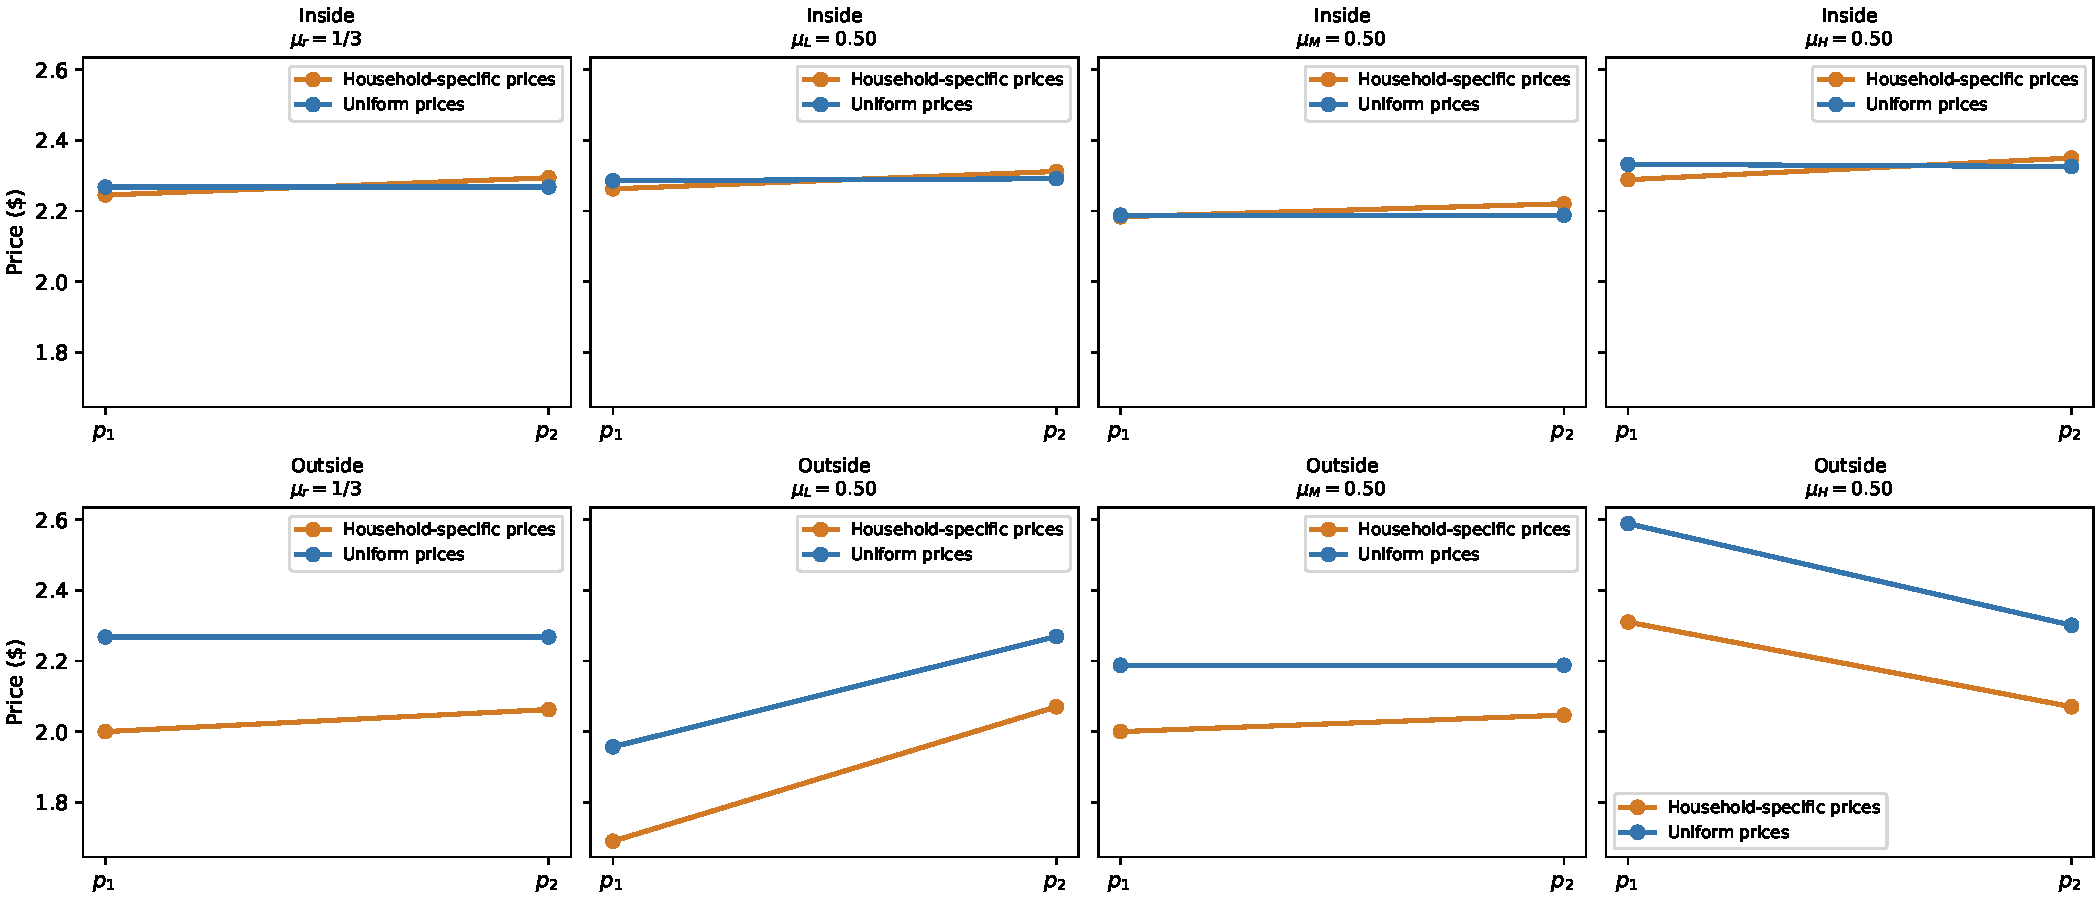
\includegraphics[width=.9\linewidth,height=.68\textheight,keepaspectratio]{assets/current/gamma-first.pdf}
\caption{Expected first-period offered prices, averaged over type when type is known.}
\label{fig:gamma-first}
\end{figure}
%\begin{figure}[htbp]
%\centering
%\includegraphics[width=\linewidth,height=.72\textheight,keepaspectratio]{assets/results/gamma_uncertainty/terminal_prices.pdf}
%\caption{Expected terminal offered prices, averaging over type and first-period purchase outcomes.}
%\label{fig:gamma-terminal_prices}
%\end{figure}
%\FloatBarrier
\begin{figure}[htbp]
\centering
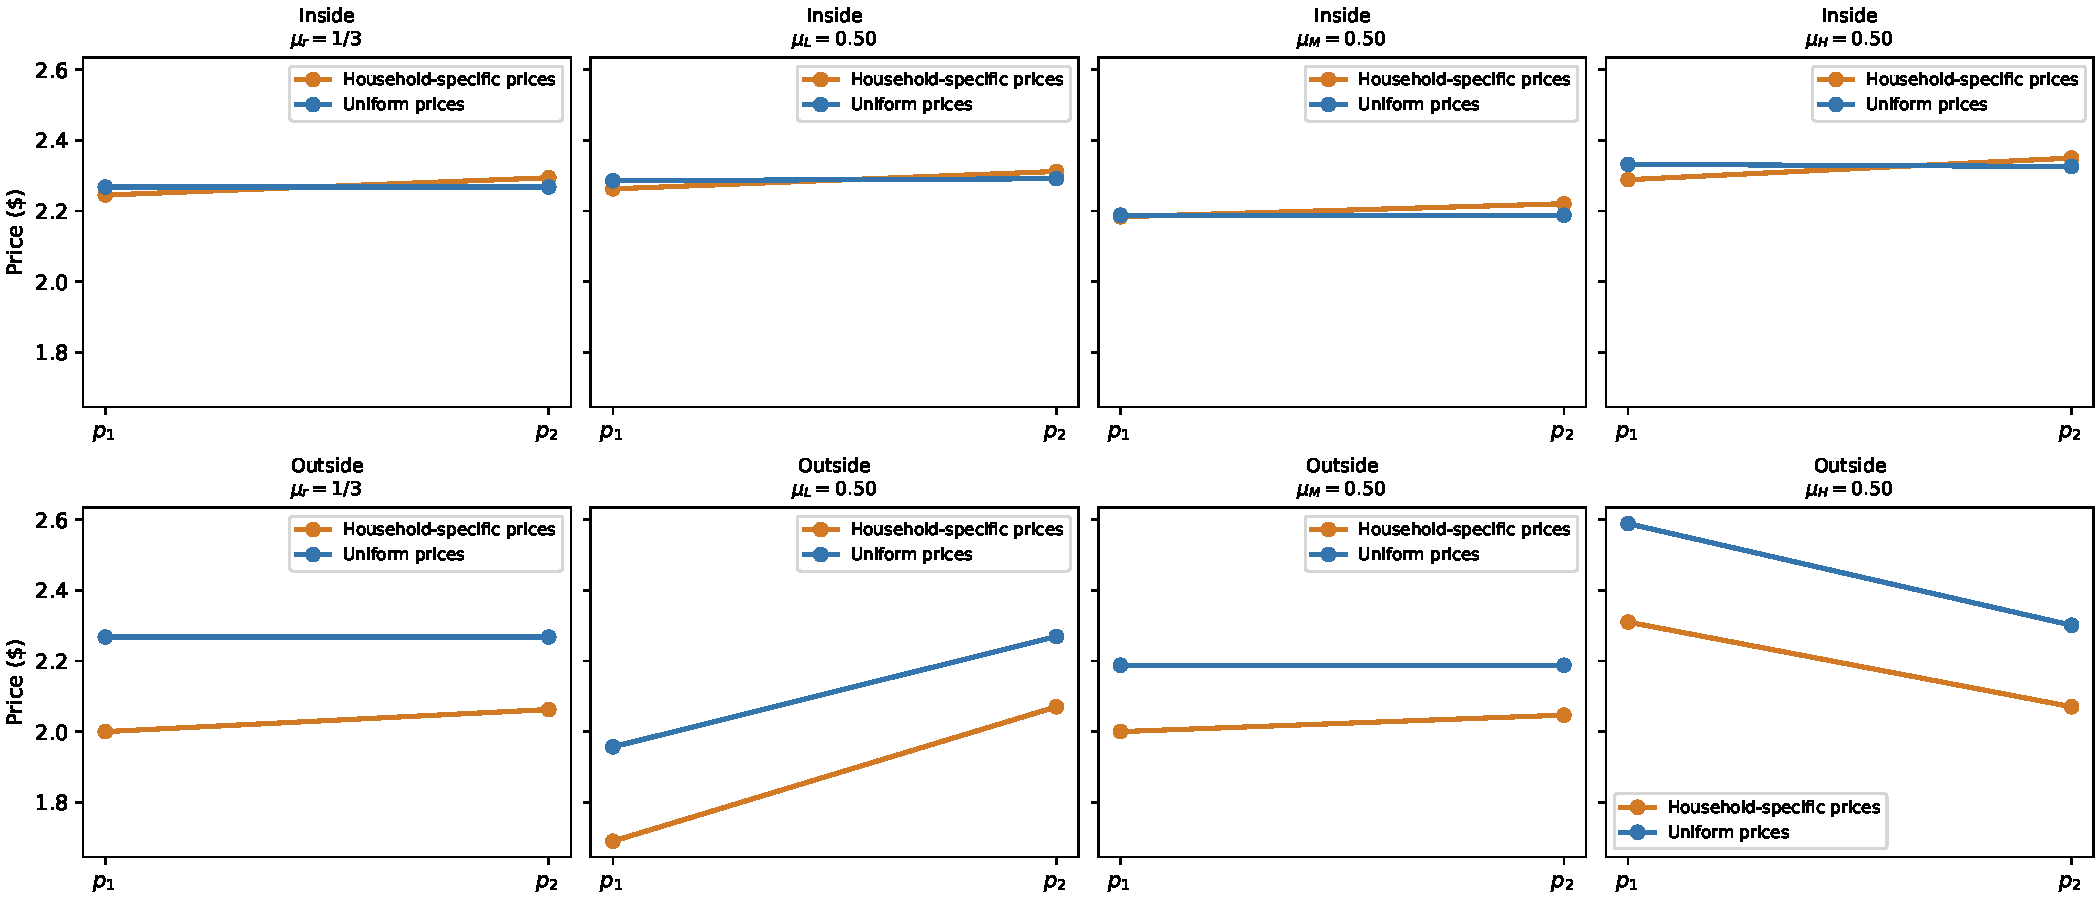
\includegraphics[width=.9\linewidth,height=.68\textheight,keepaspectratio]{assets/current/gamma-terminal.pdf}
\caption{Expected terminal offered prices, averaged over first-period outcomes and type.}
\label{fig:gamma-terminal}
\end{figure}
%
%\section{Additional Data Details}
%\label{app:data}
%
%
%\section{Empirical Demand and Estimation Derivations}
%\label{app:estimation}
%
%\subsection{Parameters and Purchase Histories}
%The estimated parameter vector is
%\begin{equation}
% \theta=(\beta_0,\beta_{\mathrm{berry}},\beta_{\mathrm{plain}},
% \mu_\alpha,\sigma_\alpha,\mu_\gamma,\sigma_\gamma,\mu_\phi,\sigma_\phi)'.
%\end{equation}
%The main-text history measures correspond to the separate-history specification
%in the estimator. For an adjacent prior purchase week,
%\begin{align}
% N_{ijt}&=\sum_{k\ne j}w_{ik,t-1}\\
% &=\frac{\sum_{k\ne j}y_{ik,t-1}}{Q_{i,t-1}}
% =1-\frac{y_{ij,t-1}}{Q_{i,t-1}}.
%\end{align}
%If the prior basket contains only flavor $k$, then
%\begin{equation}
% N_{ijt}=\mathbf{1}\{k\ne j\}.
%\end{equation}
%The share measure therefore reduces to the slides' switching indicator for
%single-flavor baskets, while retaining mixed-flavor observations.
%Equation~\eqref{eq:novelty-example} illustrates the calculation for a mixed basket.
%The stock $H_{ijt}$ sums weekly own-flavor shares without depreciation or
%normalization by the number of previous weeks. Each observed purchase week adds
%one unit across flavors:
%\begin{equation}
% \sum_{j\in\mathcal J}H_{ijt}
% =\#\{s\in\mathcal H_i:s<t\}.
%\end{equation}
%Histories are constructed before likelihood exclusions. Current purchases update
%the stock only after the current week's predictors are recorded.
%
%\subsection{Logit Probabilities}
%For $j\in\mathcal A_{it}^0$, the probability that utility from $j$ exceeds utility
%from all other alternatives is
%\begin{align}
% P_{ijt}(\nu;\theta)
% &=\Pr\!\left(\varepsilon_{ikt}-\varepsilon_{ijt}
% \le V_{ijt}-V_{ikt}\ \text{for all }k\ne j\mid\nu\right)\\
% &=\int_{-\infty}^{\infty} f(e)
% \prod_{k\ne j}F(e+V_{ijt}-V_{ikt})\,de.
%\end{align}
%For Type-I extreme-value shocks,
%\begin{equation}
% F(e)=\exp(-e^{-e}),\qquad f(e)=e^{-e}\exp(-e^{-e}).
%\end{equation}
%Writing $A=\sum_{k\in\mathcal A_{it}^0}\exp(V_{ikt}-V_{ijt})$ and using $z=e^{-e}$,
%\begin{align}
% P_{ijt}(\nu;\theta)
% &=\int_{-\infty}^{\infty}e^{-e}\exp(-Ae^{-e})\,de\\
% &=\int_0^\infty e^{-Az}\,dz
% =\frac{1}{A}\\
% &=\frac{\exp(V_{ijt})}{\sum_{k\in\mathcal A_{it}^0}\exp(V_{ikt})}.
%\end{align}
%Setting $V_{i0t}=0$ gives the denominators in the main text.
%
%\subsection{Weekly Counts and the Panel Likelihood}
%Conditional on type and the observed pre-choice history, the multinomial
%probability of a weekly count vector is
%\begin{equation}
% f(y_{it}\mid\nu;\theta)
% =\frac{M_{it}!}{\prod_{j\in\mathcal A_{it}^0}y_{ijt}!}
% \prod_{j\in\mathcal A_{it}^0}P_{ijt}(\nu;\theta)^{y_{ijt}}.
%\end{equation}
%The product of factorial terms is independent of $\theta$. Dropping this factor,
%\begin{align}
% L_i(\nu;\theta)
% &=\prod_{t\in\mathcal T_i}\prod_{j\in\mathcal A_{it}^0}
% P_{ijt}(\nu;\theta)^{y_{ijt}},\\
% \ell_i(\nu;\theta)
% &=\sum_{t\in\mathcal T_i}\sum_{j\in\mathcal A_{it}^0}
% y_{ijt}\log P_{ijt}(\nu;\theta).
%\end{align}
%For single-choice observations this reduces to
%\begin{equation}
% L_i(\nu;\theta)=\prod_{t\in\mathcal T_i}P_{i,x_{it},t}(\nu;\theta).
%\end{equation}
%Because the same type persists throughout the panel, integrate after taking
%the product over periods:
%\begin{align}
% L_i(\theta)&=\int\exp\{\ell_i(\nu;\theta)\}\varphi_3(\nu)\,d\nu,\\
% \widehat L_i(\theta)&=\frac{1}{R}\sum_{r=1}^R
% \exp\{\ell_i(\nu_{ir};\theta)\},\qquad R=128.
%\end{align}
%
%\subsection{Stable Objective Evaluation}
%For each consumer and simulation draw, let
%\begin{align}
% \ell_{ir}(\theta)
% &=\sum_t\sum_{j\in\mathcal A_{it}^0}y_{ijt}
% \left[V_{ijt}(\nu_{ir};\theta)
% -\log\!\left(\sum_{k\in\mathcal A_{it}^0}e^{V_{ikt}(\nu_{ir};\theta)}\right)\right],\\
% m_i(\theta)&=\max_{1\le r\le R}\ell_{ir}(\theta).
%\end{align}
%Then
%\begin{align}
% \log\widehat L_i(\theta)
% &=m_i(\theta)+\log\left(\sum_{r=1}^R
% e^{\ell_{ir}(\theta)-m_i(\theta)}\right)-\log R,\\
% Q_R(\theta)&=-\sum_i\log\widehat L_i(\theta).
%\end{align}
%The same log-sum-exp calculation applies to the logit denominator.
%
%\subsection{Simulated Score}
%Define the posterior weight on simulation draw $r$ for consumer $i$:
%\begin{equation}
% w_{ir}(\theta)=\frac{e^{\ell_{ir}(\theta)}}{\sum_{s=1}^Re^{\ell_{is}(\theta)}}.
%\end{equation}
%Differentiating the log simulated likelihood gives
%\begin{align}
% \nabla_\theta\log\widehat L_i(\theta)
% &=\sum_{r=1}^R w_{ir}(\theta)\nabla_\theta\ell_{ir}(\theta),\\
% \nabla_\theta\ell_{ir}(\theta)
% &=\sum_t\sum_{j\in\mathcal A_{it}^0}
% [y_{ijt}-M_{it}P_{ijt}(\nu_{ir};\theta)]
% \nabla_\theta V_{ijt}(\nu_{ir};\theta),\\
% \nabla_\theta Q_R(\theta)
% &=-\sum_i\sum_{r=1}^R w_{ir}(\theta)\nabla_\theta\ell_{ir}(\theta).
%\end{align}
%
%\subsection{Random-Coefficient Moments}
%Under the specified independent distributions,
%\begin{align}
% \E[\alpha_i]&=-\exp(\mu_\alpha+\sigma_\alpha^2/2),\\
% \Var(\alpha_i)&=(e^{\sigma_\alpha^2}-1)e^{2\mu_\alpha+\sigma_\alpha^2},\\
% \E[\gamma_i]&=\mu_\gamma,\qquad \Var(\gamma_i)=\sigma_\gamma^2,\\
% \E[\phi_i]&=\mu_\phi,\qquad \Var(\phi_i)=\sigma_\phi^2.
%\end{align}
%
%
%
%\section{Additional Results}
%\label{app:results}
%
%\subsection{Controlled Demand Estimates}
%The controlled specification augments deterministic utility with the fitted
%price residual:
%\begin{equation}
% V_{ijt}^{\mathrm{CF}}=V_{ijt}+\rho\widehat v_{ijt}.
%\end{equation}
%Here $\widehat v_{ijt}$ is the residual from the flavor-specific price equation
%using the same-week mean price outside the household's DMA as instrument and
%week and DMA fixed effects. The no-control specification sets $\rho=0$.
%\input{assets/results/demand_controlled/first_stage.tex}
%\FloatBarrier
%
%\input{assets/results/demand_controlled/estimates.tex}
%\FloatBarrier
%\input{assets/results/demand_controlled/implied_wtp.tex}
%\FloatBarrier
%\begin{figure}[htbp]
%\centering
%\includegraphics[width=\linewidth,height=.65\textheight,keepaspectratio]{assets/results/demand_controlled/history_distributions.pdf}
%\caption{Novelty and habit distributions with price controls.}
%\label{fig:controlled-distributions}
%\end{figure}
%\FloatBarrier
%\subsection{Empirical Information Friction: Detailed Results}
%\input{assets/results/empirical_information/plain/results.tex}
%\FloatBarrier
%\begin{figure}[htbp]
%\centering
%\includegraphics[width=\linewidth,height=.65\textheight,keepaspectratio]{assets/results/empirical_information/plain/first_prices.pdf}
%\caption{Plain: first prices under fixed beliefs and known novelty type.}
%\label{fig:empirical-plain-first_prices}
%\end{figure}
%\FloatBarrier
%\begin{figure}[htbp]
%\centering
%\includegraphics[width=\linewidth,height=.65\textheight,keepaspectratio]{assets/results/empirical_information/plain/terminal_prices.pdf}
%\caption{Plain: terminal prices under fixed beliefs and known novelty type.}
%\label{fig:empirical-plain-terminal_prices}
%\end{figure}
%\FloatBarrier
%\input{assets/results/empirical_information/berry/results.tex}
%\FloatBarrier
%\begin{figure}[htbp]
%\centering
%\includegraphics[width=\linewidth,height=.65\textheight,keepaspectratio]{assets/results/empirical_information/berry/first_prices.pdf}
%\caption{Berry: first prices under fixed beliefs and known novelty type.}
%\label{fig:empirical-berry-first_prices}
%\end{figure}
%\FloatBarrier
%\begin{figure}[htbp]
%\centering
%\includegraphics[width=\linewidth,height=.65\textheight,keepaspectratio]{assets/results/empirical_information/berry/terminal_prices.pdf}
%\caption{Berry: terminal prices under fixed beliefs and known novelty type.}
%\label{fig:empirical-berry-terminal_prices}
%\end{figure}
%\FloatBarrier
%
%
%\begin{figure}[htbp]
%\centering
%\includegraphics[width=\linewidth,height=.65\textheight,keepaspectratio]{assets/results/pricing/berry/discounts_by_household_type.pdf}
%\caption{Berry: offers by household type}
%\label{fig:household-type-berry}
%\end{figure}
%\FloatBarrier
%\begin{figure}[htbp]
%\centering
%\includegraphics[width=\linewidth,height=.65\textheight,keepaspectratio]{assets/results/pricing/plain/discounts_by_household_type.pdf}
%\caption{Plain: offers by household type}
%\label{fig:household-type-plain}
%\end{figure}
%\FloatBarrier
%
%
%
\end{document}
